% The Catholic University of America PhD Dissertation Template (2021/03/23)

% This is a dissertation template for The Catholic University of America based of the Turabian Formatting for Theses and Dissertations.

% * CUA's Dissertation handbook can be found at https://graduate-studies.catholic.edu/doctoral/handbook.html

% * Developed using the turabian-formatting package (2018/08/01), available through CTAN: http://www.ctan.org/pkg/turabian-formatting

% ## Additional document class formatting options:

% natbib commands was used for the bibliography and references. 
% * Citation commands can be found at https://www.overleaf.com/learn/latex/natbib_citation_styles

% Solar Physics Journal bibligraphy format was used 
% * For instructions of bibliography access https://www.springer.com/journal/11207/submission-guidelines#Instructions%20for%20Authors_Additional%20Instructions

% ## Additional commands
% * raggedright: ragged right formatting without hyphenations
% * authordate: support for the author-date citation style
% * endnotes: support for endnotes

% This template can also be found at GitHub page at https://github.com/luiz0992/thesis_template_cua
% Adapted by Luiz F. G. dos Santos (2021/03/23)

\documentclass[12pt]{turabian-thesis}
\usepackage{graphicx}
\usepackage{url}
\usepackage{lipsum}
\usepackage{blindtext}
\usepackage{longtable}
\usepackage{pdflscape}
\usepackage{graphicx}
\usepackage{verbatim}
\usepackage{color}
\usepackage{booktabs}
\usepackage{hyperref}
\usepackage{natbib}
\usepackage{tabularx}
\usepackage{amsmath}
\usepackage{mathtools}
\usepackage{array}
\usepackage{multirow}
\usepackage[normalem]{ulem}
\usepackage{xspace}
\usepackage{xcolor}
\usepackage[varg]{txfonts}
\usepackage{colortbl,dcolumn}
\newcommand\hmmax{0}
\newcommand\bmmax{0}
\usepackage{bm}
\usepackage{ragged2e}
\usepackage{siunitx}
\usepackage{cancel}
\setcounter{secnumdepth}{3}
\setcounter{tocdepth}{2}
\usepackage{dingbat}
\usepackage{amssymb}% http://ctan.org/pkg/amssymb
\usepackage{pifont}% http://ctan.org/pkg/pifont
\newcommand{\cmark}{\ding{51}}%
\newcommand{\xmark}{\ding{55}}%
\makeatletter
    \renewcommand*{\l@section}{%
        \ifnum \c@tocdepth >\z@ \vskip \tf@singlelineskip \fi
        \@dottedtocline{1}{1.25in}{0.5in}}
    \renewcommand*{\l@subsection}{%
        \ifnum \c@tocdepth >\z@ \vskip \tf@singlelineskip \fi
        \@dottedtocline{2}{1.75in}{0.5in}}
\makeatother
% Information for title page
\title{SEARCH FOR DARK MATTER PRODUCED IN ASSOCIATION WITH MONOTOP IN THE FULLY
LEPTONIC CHANNEL IN PROTON-PROTON COLLISIONS AT 13 TEV WITH THE COMPACT
MUON SOLENOID EXPERIMENT}

%\subtitle{A Template based on Turabian's \emph{A Manual for Writers}, 9th edition}
\author{Rishabh Uniyal}

%FILL OUT YOUR CORRECT INFORMATION HERE!!!
\authorinfo{Ph.D., The Catholic University of America, 2022}
\department{Department of Physics}
\school{School of Arts and Science}
\institution{The Catholic University of America}
\location{Washington, D.C.}
\degreework{Doctor of Philosophy}

%For List of figures and table titles excluded word from capitalization 
% \Addlcwords{the of into in to a at on and is for}

% \makenomenclature

\begin{document}

% \renewcommand{\thepage}{\roman{page}}

\frontmatter
\maketitle
\begin{center}
    \MyTitle \\
    \vspace*{0.5\baselineskip}
    \MyAuthor~[TITLE CONFERRED UPON GRADUATION] \\
    \vspace*{0.5\baselineskip}
    Director: [Aaron Dominguez] [Professor]
\end{center}
\thispagestyle{empty}

\begingroup
\renewcommand{\clearpage}{}
\singlespacing


% \chapter*{ABSTRACT}
\vspace*{\stretch{1}} 

abstracts
\noindent
% INDEX WORDS: Georgia Southern, Thesis, ETD, Lorem ipsum.
\vspace*{\stretch{4}}
\thispagestyle{empty}

\endgroup



\PrintCommitteeInfoPage{[AUTHOR'S NAME]}{Dr. Aaron Dominguez}{Dr. Rachel Bartek}{Dr. Grzegorz Kalicy}

\chapter{DEDICATION}
\begin{center}
	\vspace*{\stretch{1}}
	
	[Optional Text]
	
	\vspace*{\stretch{4}}
\end{center}

\begin{center}
	\vspace*{\stretch{1}}
	
	\begin{FlushLeft}
	\textit{``Dedicated to my entire Uniyal clan”}\\
	\end{FlushLeft}
	\begin{FlushRight}
    [Author of the citation]
	\end{FlushRight}

	\begin{FlushLeft}
	\textit{``A inspirational citation"}
	\end{FlushLeft}
	\begin{FlushRight}
    [Author of the inspirational citation]
	\end{FlushRight}

	
	\vspace*{\stretch{4}}
\end{center}

\chapter{ACKNOWLEDGEMENTS}
\vspace{\baselineskip}
\doublespacing


I would like to thank a lot of people in this journey, I would like to start by thanking myself for being brave, for taking risks, for motivating myself to keep fighting and finishing this dissertation
\tableofcontents 
\listoffigures
\listoftables
\mainmatter

\chapter{Introduction}
\label{chapter:introduction}

%\section{An Interesting Section}
%\label{section:interesting_section}

The Standard Model (SM) of Particle Physics is one of the most complete and versatile theories which describes the fundamental particles and the forces with which they interact. The SM has been successful at describing many features of the nature that we have observed in our experiments. From the precise measurement of the electron's magnetic dipole moment to the discovery of the Higgs Boson. The predictions of the SM have just been too good. While the SM may has been really successful, there are some phenomenon like absence of the description of Dark Matter (DM) in the SM which prevents it from taking the title of the most complete and unified theory.

Dark Matter  is a form of material that neither emits, absorbs or reflects any Electromagnetic Radiation. It does seem to have mass given its Gravitational effects. Dark Matter contributes to around 24\% of the total mass energy of the universe (or 5 times the mass of ordinary matter) but does not interact directly with light, so we have not observed it yet. Astrophysical observations like Gravitational Lensing [2] (bending of light coming from distant galaxies by massive galaxies or galaxy clusters) and motion of galaxies at speeds so high for ordinary matter to sustain, Galaxy Cluster Collisions [3] and Dark Matter seeded Galaxy formations [4] have provided evidence for the presence of Dark Matter.

There are different ways in which Dark Matter could be detected-- direct detection, indirect detection and making Dark Matter on the Earth and then detecting it. The Large Hadron Collider (LHC) collides proton beams at the highest energy in the world. The proton beams collide at four main interaction points at the LHC. At each interaction point is a detector. In this thesis we will show the search for Dark Matter, based on the proton-proton collision data recorded by the Compact Muon Solenoid (CMS) experiment at the LHC.



\begin{quotation}
    \noindent Here is a block quotation---a passage from a text you found insightful and wanted to share with others. Maybe it is from a journal article, website, or book. Irrespective, it should support the argument being made.\footnote{A citation for the quoted material.}
\end{quotation}

%Maybe a sentence or two that bring the argument and evidence together.\citep{dos_santos_2020}

Check appendix \ref{appendix: chapter1}

\begin{figure} [ht]
\centering
         
\includegraphics[width=0.9\textwidth,clip=]{Figures/Introduction/CUA_logo.png}
         \caption{CUA Logo}
         \label{CUA-logo-1}
\end{figure}


\section{Another Insightful Section}
\label{section:another_interesting_section}

More ideas that really make this a great paper. Maybe a footnote or two.\footnote{Some peripheral thoughts that belong in a note.}

\chapter{Theoretical Motivations for Dark Matter Search}
\label{chapter:two}
\section{An Interesting Section}

Great thoughts that further your argument. This includes lots of strong evidence presented throughout several paragraphs, each accompanied by necessary citations.
\begin{quotation}
    \noindent Here is a block quotation---a passage from a text you found insightful and wanted to share with others. Maybe it is from a journal article, website, or book. Irrespective, it should support the argument being made.\footnote{A citation for the quoted material.}
\end{quotation}

Check appendix \ref{appendix: chapter2}
%Maybe a sentence or two that bring the argument and evidence together.\citep{dos_santos_2020}

\begin{table}[h!]
  \centering
  \caption{Very imporant table.}
  \label{tab:average_channels}
  \begin{tabular}{cc}
    \toprule
     AIA channel (\AA) &  Scaling unit [DN/s/pixel] \\
     \midrule
      94 &   10  \\
      131 &   80  \\
      171 & 2000  \\
      193 & 3000  \\
      211 & 1000  \\
      304 &  500  \\
      335 &   80  \\
      \bottomrule
  \end{tabular}
\end{table}


\section{Another Insightful Section}

More ideas that really make this a great paper. Maybe a footnote or two.\footnote{Some peripheral thoughts that belong in a note.}

\chapter{The CMS Experiment at the LHC}
\label{chapter:three}
\section{The Large Hadron Collider}

The Large Hadron Collider (LHC) is the world’s largest and most powerful particle accelerator. Inside the accelerator, two highly energetic proton beams collide up to a center-of-mass energy of 14 TeV. The LHC is constructed inside a 27 km tunnel, 100 m under the ground, located partly in Switzerland and France.

At the LHC two energetic proton beams travel in opposite directions in separate beam pipes. The proton beams travel in bunches separated by 25 ns in time. The beams travel at relativistic speeds and collide at four major interaction points at the LHC. The LHC has four main detector experiments at each interaction point: ALICE (A Large Ion Collider Experiment), ATLAS (A Toroidal LHC Apparatus), CMS (Compact Muon Solenoid), and LHCb (Large Hadron Collider beauty). ATLAS and CMS are general purpose-detectors with broad physics objectives ranging from studying the Standard Model to searching Beyond Standard Model (BSM) physics such as Dark Matter. While ALICE and LHCb are more physics dedicated detectors, ALICE and LHCb are dedicated to heavy-ion physics and studying b-quark physics respectively.

%\begin{quotation}
%    \noindent Here is a block quotation---a passage from a text you found insightful and wanted to share with others. Maybe it is from a %journal article, website, or book. Irrespective, it should support the argument being made.\footnote{A citation for the quoted material.}
%\end{quotation}

%Check appendix \ref{appendix: chapter3}

%Maybe a sentence or two that bring the argument and evidence together.\citep{dos_santos_2020}



\section{The Compact Muon Solenoid Experiment}
\subsection{Introduction}
The Compact Muon Solenoid (CMS) is a general purpose detector located in eastern France at the Large Hadron Collider (LHC) tunnel 100 m underground. It is a general purpose detector because of its broad physics searches ranging from studying the Standard Model (SM) to searching for particles that could potentially make Dark Matter (DM). CMS is a cylindrical shaped detector with 21 m in length and 15 m in cross-sectional diameter. The three main characteristics of the CMS experiment are its compactness, accurate detection of Muon particles in the muon system and its magnetic solenoid. The superconducting magnetic solenoid at the core of the CMS detector produces a continuous magnetic field of 3.8 T which is of the order of O(5) of Earth's magnetic field (0.25 - 0.65 gaus). Such large magnetic field is required for a precise measurement of the momentum of high-energy charged particles. All CMS detector subsystems are enclosed by the magnetic solenoid, the muon system, on the other hand, is on the outside. Muons are the particles that are directly detected by the CMS, with a special property that they neither stop nor decay within the boundaries of the detector. They undergo very little energy loss and thus act as a powerful medium to study high-energy process in the presence of high background.
The CMS detector is cylindrical shaped with an onion like structure, having several concentric layers of subsystems. These subsystems help prepare "photographic images" of each collision event by determining the properties of the particles in the collision. CMS has the following basic subsystems ordered from innermost to outermost:

\begin{enumerate}
    \item Silicon Tracker
    \item Electromagnetic Calorimeter
    \item Hadronic Calorimeter
    \item Superconducting Solenoid Magnet
    \item Muon System
    
    
\end{enumerate}
The CMS detector can detect 5 general categories of particles as shown in the figure below:
 \begin{enumerate}
    \item Electrons
    \item Photons
    \item Charged Hadrons
    \item Neutral Hadrons
    \item Muons
\end{enumerate}

\begin{figure} [ht]
\centering
         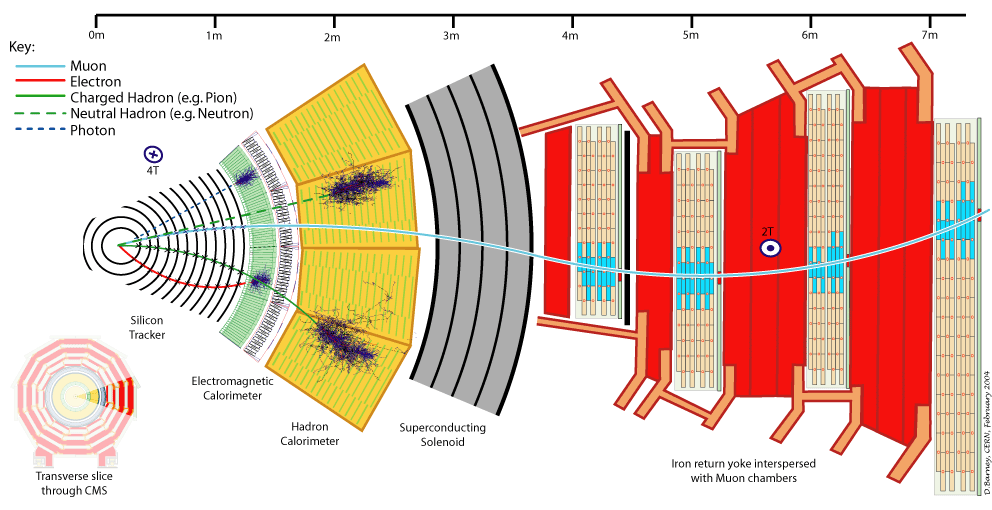
\includegraphics[width=0.9\textwidth,clip=]{thesis_template_cua/Figures/CMS_LHC_chapter/CMSSlice.png}
         \caption[#CMS Slice]{This Figure shows the cross-sectional slice of the CMS detector. Here we have shown the different sub-systems of CMS, trajectories and energy deposits of the 5 general categories of particles detected by CMS by one or more of its sub-systems}
         \label{cms_slice}
\end{figure}
%More ideas that really make this a great paper. Maybe a footnote or two.\footnote{Some peripheral thoughts that belong in a note.}
\subsection{Coordinate System}


\subsection{Silicon Tracker}

\subsection{Electromagnetic Calorimeter}

\subsection{Hadronic Calorimeter}

\subsection{Solenoid Magnet}

\subsection{Muon System}

\subsubsection{DT}

\subsubsection{RPC}

\subsubsection{CSC}

\subsection{Trigger System}
\chapter{Theoretical Foundations of Monotop Analysis}
\label{chapter:four}
This Chapter will focus on the explaining the theory behind the monotop analysis and the importance of the top quark.
\section{Monotop Analysis}

Great thoughts that further your argument. This includes lots of strong evidence presented throughout several paragraphs, each accompanied by necessary citations.
\begin{quotation}
    \noindent Here is a block quotation---a passage from a text you found insightful and wanted to share with others. Maybe it is from a journal article, website, or book. Irrespective, it should support the argument being made.\footnote{A citation for the quoted material.}
\end{quotation}
%Maybe a sentence or two that bring the argument and evidence together.\citep{dos_santos_2020}



\section{The Top quark}

The top quark was discovered the Fermilab Tevatron almost 25 years ago. It is the weak isospin partner of the bottom quark. Its discovery resulted in completion of the three generation structure of the standard model (SM). The top quark mass was measured to be $m_{t} = 176 \pm 13$ GeV, a charge of 2/3 times the charge on the electron and a lifetime of $5 \times 10^{-25} s$ making it the heaviest of all the fermions known till date in the standard model. Because of it's large mass and correspondingly short lifetime it behaves differently than other quarks. 

The top quark decays before it hadronizes, passing its information to the decay products. Therefore making it possible to infer its properties from the decay products in the detector. The top quark decays into a a bottom quark and a W boson, and since the W boson is an unstable particle it decays into a quark anti-quark pair of different flavors (hadronic decay channel) or to a charged lepton and a neutrino (leptonic decay channel) with the following branching ratios.

\begin{table}[h!]
  \centering
  \caption{}
  \label{tab:average_channels}
  \begin{tabular}{cc}
    \toprule
     Decay channel &  Branching ratio \\
     \midrule
      $W^{\pm} \rightarrow q\Bar{q'}$ &   $68.32\%$  \\
      $W^{\pm} \rightarrow e^{\pm} \Bar{\nu_{e}}$ &   $10.46\%$  \\
      $W^{\pm} \rightarrow \mu^{\pm} \Bar{\nu_{\mu}}$ &   $10.50\%$  \\
      $W^{\pm} \rightarrow \tau^{\pm} \Bar{\nu_{\tau}}$ &   $10.75\%$  \\
      \bottomrule
  \end{tabular}
\end{table}

As the top quark decays into a W boson and a bottom quark, it's evident that the hadronic and leptonic decay probabilities of the top quark will be proportional to the hadronic and leptonic decay probabilities of the W boson. So, it can be implied from the above table that, around 70\% of times the top quark decays into three quarks (two quarks from W boson and one bottom quark) which further hadronize to produce jets. While around 30\% of the times the top quark would decay leptonically to a lepton, its corresponding lepton neutrino and a bottom quark. In this thesis we will be exploring the leptonic channel for the search for Dark Matter (DM), so our final state signature would a lepton, its corresponding neutrino and a jet coming from a bottom quark.

In accordance with the SM, at the LHC, top quarks are predominantly produced in pairs ($t \Bar{t}$) through strong interactions and as single top via the electroweak interaction. In the following section we will be looking at the production of a single top quark (Monotop) in association with missing transverse energy due to the two DM candidates, as an extension to the SM. 


\section{The Monotop Model}
\chapter{Statistical Framework of Monotop Analysis}
\label{chapter:five}
This chapter will explain the analysis strategy for the monotop analysis in the leptonic channel
\section{Analysis Strategy}\label{analysis-strategy}

This section will detail the analysis strategy for the search of leptonically decaying mono-top signature. As we have seen in section \ref{monotopmodel}, the final state signature of the mono-top events includes missing transverse energy and leptonic or hadronic decay of the top quark. In this analysis since we focus on the leptonic decay of mono-top as the final state signature along side the missing transverse energy. The theoretical mono-top models being tested in this analysis expects a large missing transverse energy due to the recoil of the top quark against the higher mass of the dark matter mediator, which further decays into two invisible dark matter candidates.

The final state signature we are targeting is the presence of a large missing energy (from the proposed DM candidates and lepton neutrino from the single top quark decay) and the presence of a b-tagged jet alongside a prompt lepton, called leptonic decay. However there are several SM processes that produce the same final state signature. We will briefly detail them below.

% \begin{figure} [tpb]
% \centering
%          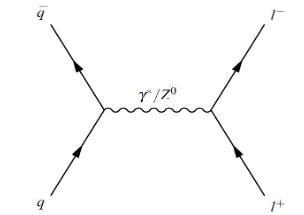
\includegraphics[width=0.45\textwidth,clip=]{thesis_template_cua/Figures/ch5_analysis/DY.png}
%          \vspace*{10mm}
%          \caption[Tree-Level Feynman]{ [Left]:  }
%          \label{analysis:dy}
% \end{figure}
\begin{figure}%
    \centering
    \subfloat[\centering Drell-Yan Jets]{{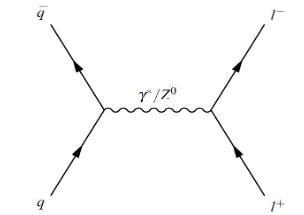
\includegraphics[width=5cm]{thesis_template_cua/Figures/ch5_analysis/DY.png} }}%
    \qquad
    \subfloat[\centering W(l $\nu$) Jets]{{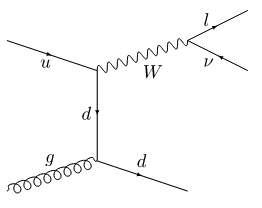
\includegraphics[width=5cm]{thesis_template_cua/Figures/ch5_analysis/Wjets.png} }}%
    \qquad
    \subfloat[\centering $t \bar{t}$ Jets]{{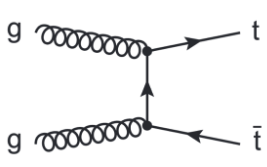
\includegraphics[width=5cm]{thesis_template_cua/Figures/ch5_analysis/ttbar.png} }}%
    \qquad
    \subfloat[\centering Di-Boson]{{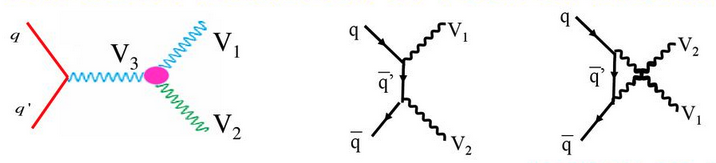
\includegraphics[width=12cm]{thesis_template_cua/Figures/ch5_analysis/diboson.png} }}%
    \caption{Leading-order Feynman diagram for a.) Drell-Yan process where a neutral Z boson decays to a lepton and miss-reconstructed lepton may result in signal like signature. b.) W boson production decaying into charged lepton and neutrino in association with jets. c.) $t\bar{t}$ production decaying into a W boson and b-jet. d.) WW, ZZ, WZ production with bosons decaying with signal like signatures.}%
    \label{analysis:dy-wjets}%
\end{figure}

The Drell-Yan process occurs when a quark and an anti-quark from separate hadrons annihilate creating a Z boson ($Z^{0}$) or a virtual photon ($\gamma^{*}$) with other jets, which further decay into a pair of oppositely charged leptons. If there is a miss-reconstruction of one of the lepton may result in signal like signature in the final state with a lepton, a B-jet and missing energy. A Leading-order Feynman diagram is shown in Figure \ref{analysis:dy-wjets}.a. The total production cross section of Drell-Yan process (see Table \ref{tab:bkg_table}) is significantly higher that the expected cross section of the signal samples (see Table \ref{tab:signal_table}) in the mono-top model. So, the Drell-Yan process is an important background to be estimated in our analysis. 

The other background of relevance is the production of W boson decaying into a lepton and a neutrino in association with other jets. This final state could possibly mimic our signal final states if one of the additional jets is mis-reconstructed as a  b-jet. Fig \ref{analysis:dy-wjets}.b  shows the Leading-order Feynman diagram for this process. In addition, the total cross section of the W boson production is significantly higher than the expected cross section of the signal in the mono-top model thus giving us an  indication that this background needs highly precise measurements.

the $t\bar{t}$ background is another background which may produce signal like signature. Fig \ref{analysis:dy-wjets}.c shows the Leading-order Feynman diagram. From table \ref{tab:bkg_table} we see that the total $t\bar{t}$ cross section is also significantly higher than the expected cross section of the signal in the mono-top model. The $t\bar{t}$ background can decay via a hadronic, semi-leptonic and di-leptonic modes. As we know that in this analysis we are looking for a final state comprising of a lepton, a b-tagged AK4 jet and missing energy, the semi-leptonic decay of $t\bar{t}$ would be the major background. In semi-leptonic decay if one the top decays hadronically producing a AK4 jet mis-tagged as a b-jet and the other decay leptonically producing a lepton, we could see a signal like signature from the $t\bar{t}$ background. The other decay mode would be a di-leptonic decay which is suppressed because of the small branching ratio. and finally, in all hadronic mode the missing energy contribution is not enough to be accounted as a signal-like signature. Figure \ref{analysis:ttbardecay} shows the decay mode branching ratios for the $t\bar{t}$ process.

The discriminating variable used in the statistical analysis is the transverse mass of the W boson.
The transverse mass is calculated by combining the information from the lepton, $p_{T}^{l}$ and the MET, $\cancel{\it{E}}_{T}$ according to the following formula:

\begin{equation}
m_{T}^{W} = \sqrt{2 p_{T}^{l} \cancel{\it{E}}_{T}(1 - cos(\Delta\phi(l - \cancel{\it{E}}_{T})))}
\end{equation}

Where $p_{T}^{l}$ is the transverse momentum of the leading lepton, $\cancel{\it{E}}_{T}$ is the missing transverse energy and $\Delta\phi(l - \cancel{\it{E}}_{T}))$ is the difference of the $\phi$ between the $\cancel{\it{E}}_{T}$ and lepton. 

The transverse mass has a distinct signature for W boson processes in which the W boson decays into a lepton $l$ and a neutrino $\nu$. For such cases in which the W boson is produced on-shell the distribution of transverse mass peaks at and around the W boson mass of 80 GeV and any larger contributions of W $\rightarrow$ l$\nu$ may come from off-shell W boson decays or due to incorrect reconstruction of the lepton and neutrino.

While for leptonic mono-top events as the missing energy contribution primarily comes from the DM candidates thus resulting in larger contributions to the transverse mass greater than the W boson mass. So, that's the reason we chose $m_{T}^{W}$ as the discriminating variable between signal and backgrounds as we expect the signal to have a large transverse mass compared to the dominating W+jets and $t\overline{t}$ backgrounds which have transverse mass closer W-boson mass. Since the W+Jets and $t\bar{t}$ + Jets are the major backgrounds in the leptonic channel, we create signal and control regions to determine the signal contribution and normalization of the W+Jets and $t\bar{t}$ backgrounds. These regions are distinguished based on the number of b-tagged AK4 jets in the event. 
\begin{figure} [tpb]
\centering
         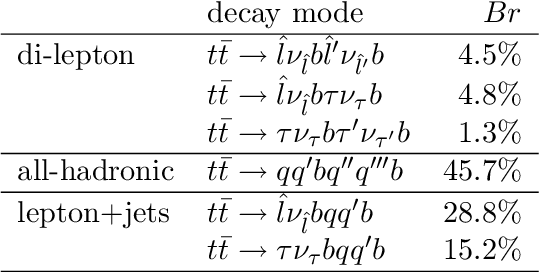
\includegraphics[width=0.6\textwidth,clip=]{thesis_template_cua/Figures/ch5_analysis/ttbardecay.png}
         \vspace*{10mm}
         \caption[ttbar decay modes]{ : Shows decay modes for a $t\bar{t}$ process }
         \label{analysis:ttbardecay}
\end{figure}

\begin{table}
\centering
\caption{Non-resonant mono-top signal samples split according to the mass of the mediator $M_{V}$ and the mass of the DM candidates $M_{\chi}$ }
\vspace{3mm}
\scalebox{1.0}{
\begin{tabular}{lll}
%\Xhline{2\arrayrulewidth}
\hline
\hline
$M_{V}\; [GeV]$  &  $M_{\chi} \; [GeV]$  &  Cross Section [pb] \\

\hline
 200 &50  &59.59\\
 195 &100 &49.31\\
 200 &150 &0.2533\\ \hline
 300 &100  &18.69\\
 295 &150  &2.373\\
 300 &300  &0.0189\\ \hline
 500 &150  &4.315\\
 495 &250  &0.704\\
 500 &500  &0.002262\\ \hline
 1000 &150  &0.3727\\
 995 &500  &0.07102\\
 1000 &1000  &5.344E-05\\ \hline
 2000 &500  &0.01297\\
 1995 &1000  &0.002655\\
 2000 &150  &0.01414\\ \hline
 1750 &150  &0.02879 \\
 1750 &700  &0.02263\\
 1700 &800  &0.0189\\ \hline
 2500 &750  &0.003237\\
 2495 &1250  &0.0006786\\ \hline
 3000 &1000  &0.0008935\\
 2995 &1500  &0.0001901\\ 
\hline

%\Xhline{2\arrayrulewidth}
\end{tabular}}
\label{tab:signal_table}
\end{table}


\begin{table}
\centering
\caption{Background samples used in the analysis for all years}
\vspace{3mm}
\scalebox{0.7}{
\begin{tabular}{ll}
%\Xhline{2\arrayrulewidth}
\hline
\hline
Sample&    Cross Section [pb] \\ \hline
ST\_s-channel\_4f\_leptonDecays\_TuneCP5\_13TeV-amcatnlo-pythia8 & 3.3024 \\ 
ST\_tW\_antitop\_5f\_inclusiveDecays\_TuneCP5\_13TeV-powheg-pythia8 & 35.85 \\ 
ST\_tW\_top\_5f\_inclusiveDecays\_TuneCP5\_13TeV-powheg-pythia8 & 35.85 \\ 
ST\_t-channel\_antitop\_4f\_InclusiveDecays\_TuneCP5\_13TeV-powheg-madspin-pythia8 & 80.95 \\ 
ST\_t-channel\_top\_4f\_InclusiveDecays\_TuneCP5\_13TeV-powheg-madspin-pythia8 & 136.02 \\ 
TTTo2L2Nu\_TuneCP5\_13TeV-powheg-pythia8 & 91.4936 \\ 
TTToHadronic\_TuneCP5\_13TeV-powheg-pythia8 & 374.292 \\ 
TTToSemiLeptonic\_TuneCP5\_13TeV-powheg-pythia8 & 365.9744 \\ \hline
DYJetsToLL\_0J\_TuneCP5\_13TeV-amcatnloFXFX-pythia8 & 5125.0 \\ 
DYJetsToLL\_1J\_TuneCP5\_13TeV-amcatnloFXFX-pythia8 & 951.4 \\ 
DYJetsToLL\_2J\_TuneCP5\_13TeV-amcatnloFXFX-pythia8 & 358.3 \\ 
DYJetsToLL\_Pt-100To250\_MatchEWPDG20\_TuneCP5\_13TeV-amcatnloFXFX-pythia8 & 94.39 \\ 
DYJetsToLL\_Pt-250To400\_MatchEWPDG20\_TuneCP5\_13TeV-amcatnloFXFX-pythia8 & 3.656 \\ 
DYJetsToLL\_Pt-400To650\_MatchEWPDG20\_TuneCP5\_13TeV-amcatnloFXFX-pythia8 & 0.4969 \\ 
DYJetsToLL\_Pt-50To100\_MatchEWPDG20\_TuneCP5\_13TeV-amcatnloFXFX-pythia8 & 395.1 \\ 
DYJetsToLL\_Pt-650ToInf\_MatchEWPDG20\_TuneCP5\_13TeV-amcatnloFXFX-pythia8 & 0.04689 \\ \hline

WJetsToLNu\_0J\_TuneCP5\_13TeV-amcatnloFXFX-pythia8 & 53300.0 \\ 
WJetsToLNu\_1J\_TuneCP5\_13TeV-amcatnloFXFX-pythia8 & 8947.0 \\ 
WJetsToLNu\_2J\_TuneCP5\_13TeV-amcatnloFXFX-pythia8 & 3335.0 \\ 
WJetsToLNu\_Pt-100To250\_MatchEWPDG20\_TuneCP5\_13TeV-amcatnloFXFX-pythia8 & 757.7 \\ 
WJetsToLNu\_Pt-250To400\_MatchEWPDG20\_TuneCP5\_13TeV-amcatnloFXFX-pythia8 & 27.53 \\ 
WJetsToLNu\_Pt-400To600\_MatchEWPDG20\_TuneCP5\_13TeV-amcatnloFXFX-pythia8 & 3.511 \\ 
WJetsToLNu\_Pt-600ToInf\_MatchEWPDG20\_TuneCP5\_13TeV-amcatnloFXFX-pythia8 & 0.5426 \\ \hline 
WW\_TuneCP5\_13TeV-pythia8 & 118.7 \\ 
WZ\_TuneCP5\_13TeV-pythia8 & 65.5443 \\ 
ZZ\_TuneCP5\_13TeV-pythia8 & 15.8274 \\ \hline

\hline

%\Xhline{2\arrayrulewidth}
\end{tabular}}
\label{tab:bkg_table}
\end{table}

%Maybe a sentence or two that bring the argument and evidence together.\citep{dos_santos_2020}

\section{Datasets}
Between 2015 and 2018, a total of 150.26 $fb^{-1}$ of data at center- of-mass energy of 13 TeV was recorded, of which 137.64 $fb^{-1}$ is used in the analysis. This loss in data occurs because of the malfunctioning of sub-detectors at different times of data collection. In order to maintain high quality data set such events from problematic detector parts are discarded.

\begin{figure} [tpb]
\centering
         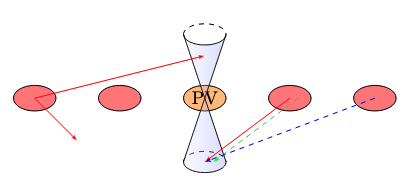
\includegraphics[width=0.6\textwidth,clip=]{thesis_template_cua/Figures/ch5_analysis/pu.png}
         \vspace*{10mm}
         \caption[PU picture]{This figure taken from \cite{Perloff:2012wpa} shows two jets coming from a primary vertex and additional soft pp interactions as red circles. The  arrows show the particles from the other collisions contribute to the jets from the primary vertex, where the colored line represent different particles.}
         \label{analysis:pu}
\end{figure}
Whenever $proton-proton$ collisions happens at the LHC, the hard scattered protons are accompanied by soft scattered $p-p$ collisions. During the reconstruction of the jets at CMS \cite{Chatrchyan:cms_detetectors} the actual $p_{T}$ of the jets is found to be different from the final-state particles that comprise the jet. This additional contribution comes from particles of the soft-scattered $p-p$ collisions near the primary vertex (PV) of the hard $p-p$ collision \cite{Perloff:2012wpa} and is called $pileup$. As these soft collisions do not contain any interesting physics, their effect must be mitigated because of their contributions to actual calorimeter deposits and tracks. The Monte Carlo (MC) \cite{Rahmat:2012fs} simulation used for modeling the backgrounds donot account for the presence of $pileup$, so we have to derive event-wise weights from the data and apply a re-weighting procedure to include the $pileup$ effects in the MC. We do this by dividing the simulated $pileup$ with the observed $pileup$ and using this ratio to re-weight the MC events.
Figure \ref{analysis:pu} shows weights associated with the additional particle contribution from the soft collisions to the jets originating from a hard collision PV for the entire Run II data.

\begin{figure}%
    \centering

    \subfloat[\centering 2016]{{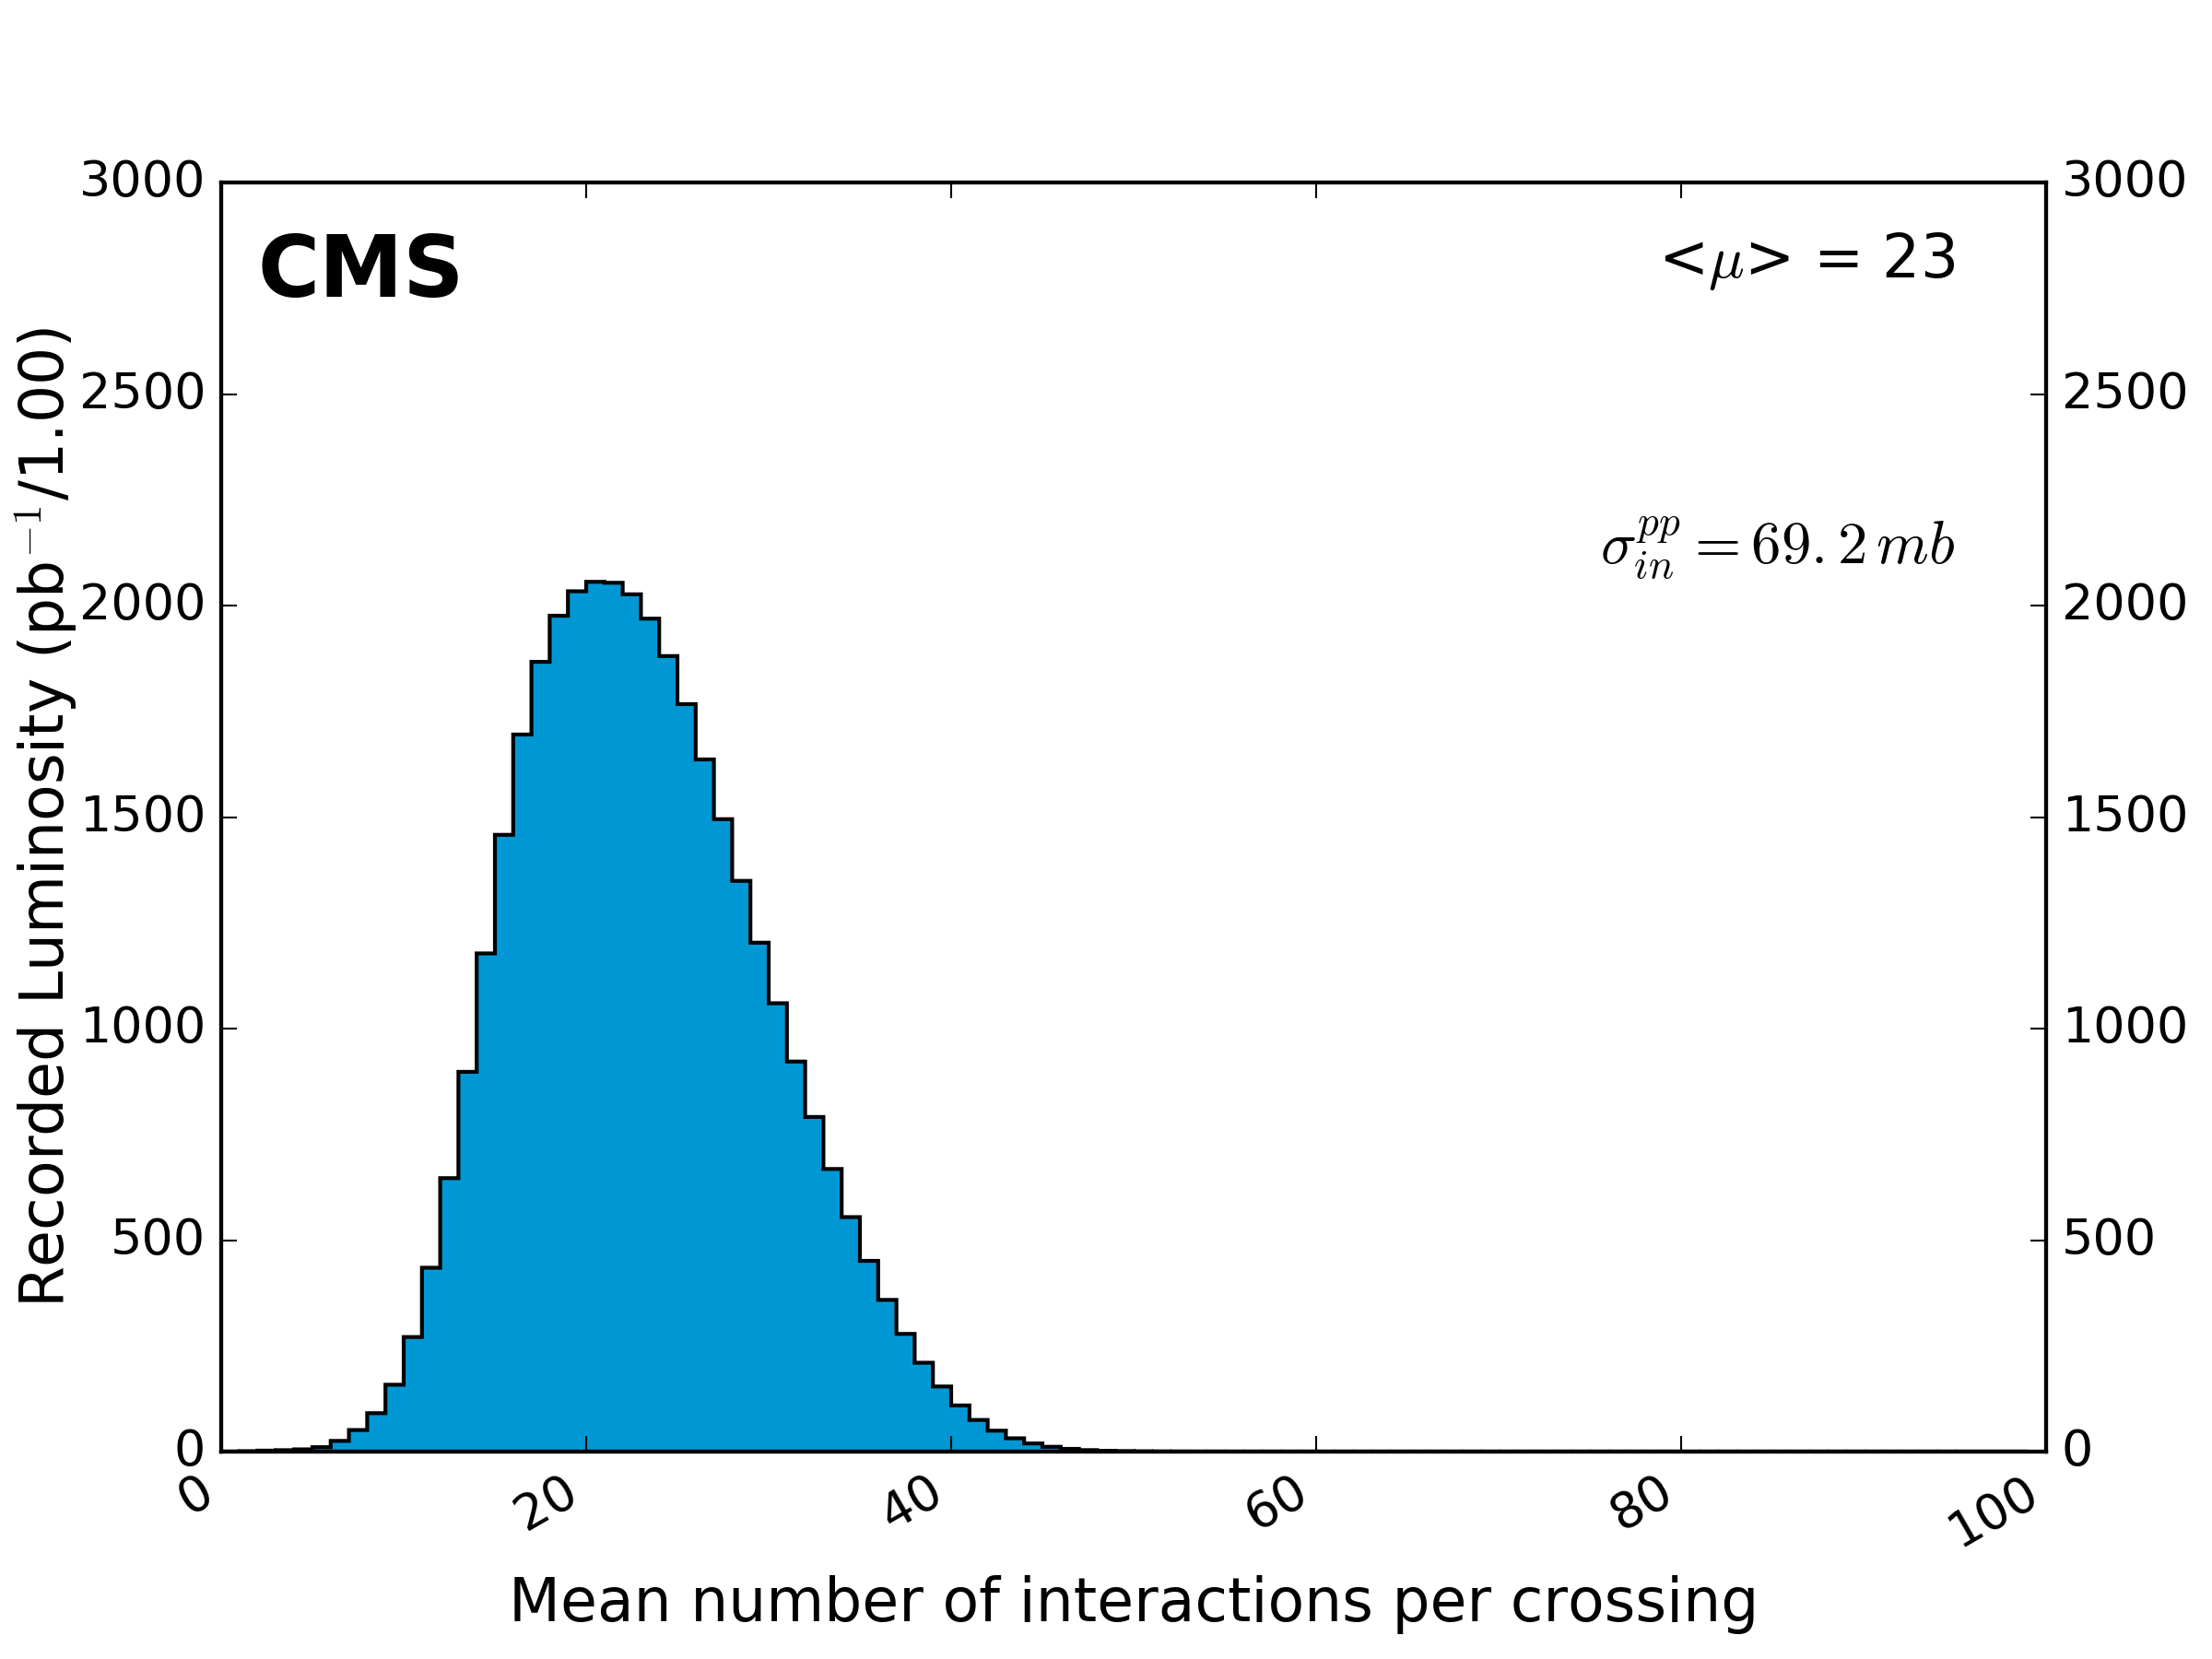
\includegraphics[width=7cm]{thesis_template_cua/Figures/ch5_analysis/pileup_pp_2016_69200_Normtag.png} }}%
    \qquad
    \subfloat[\centering 2017]{{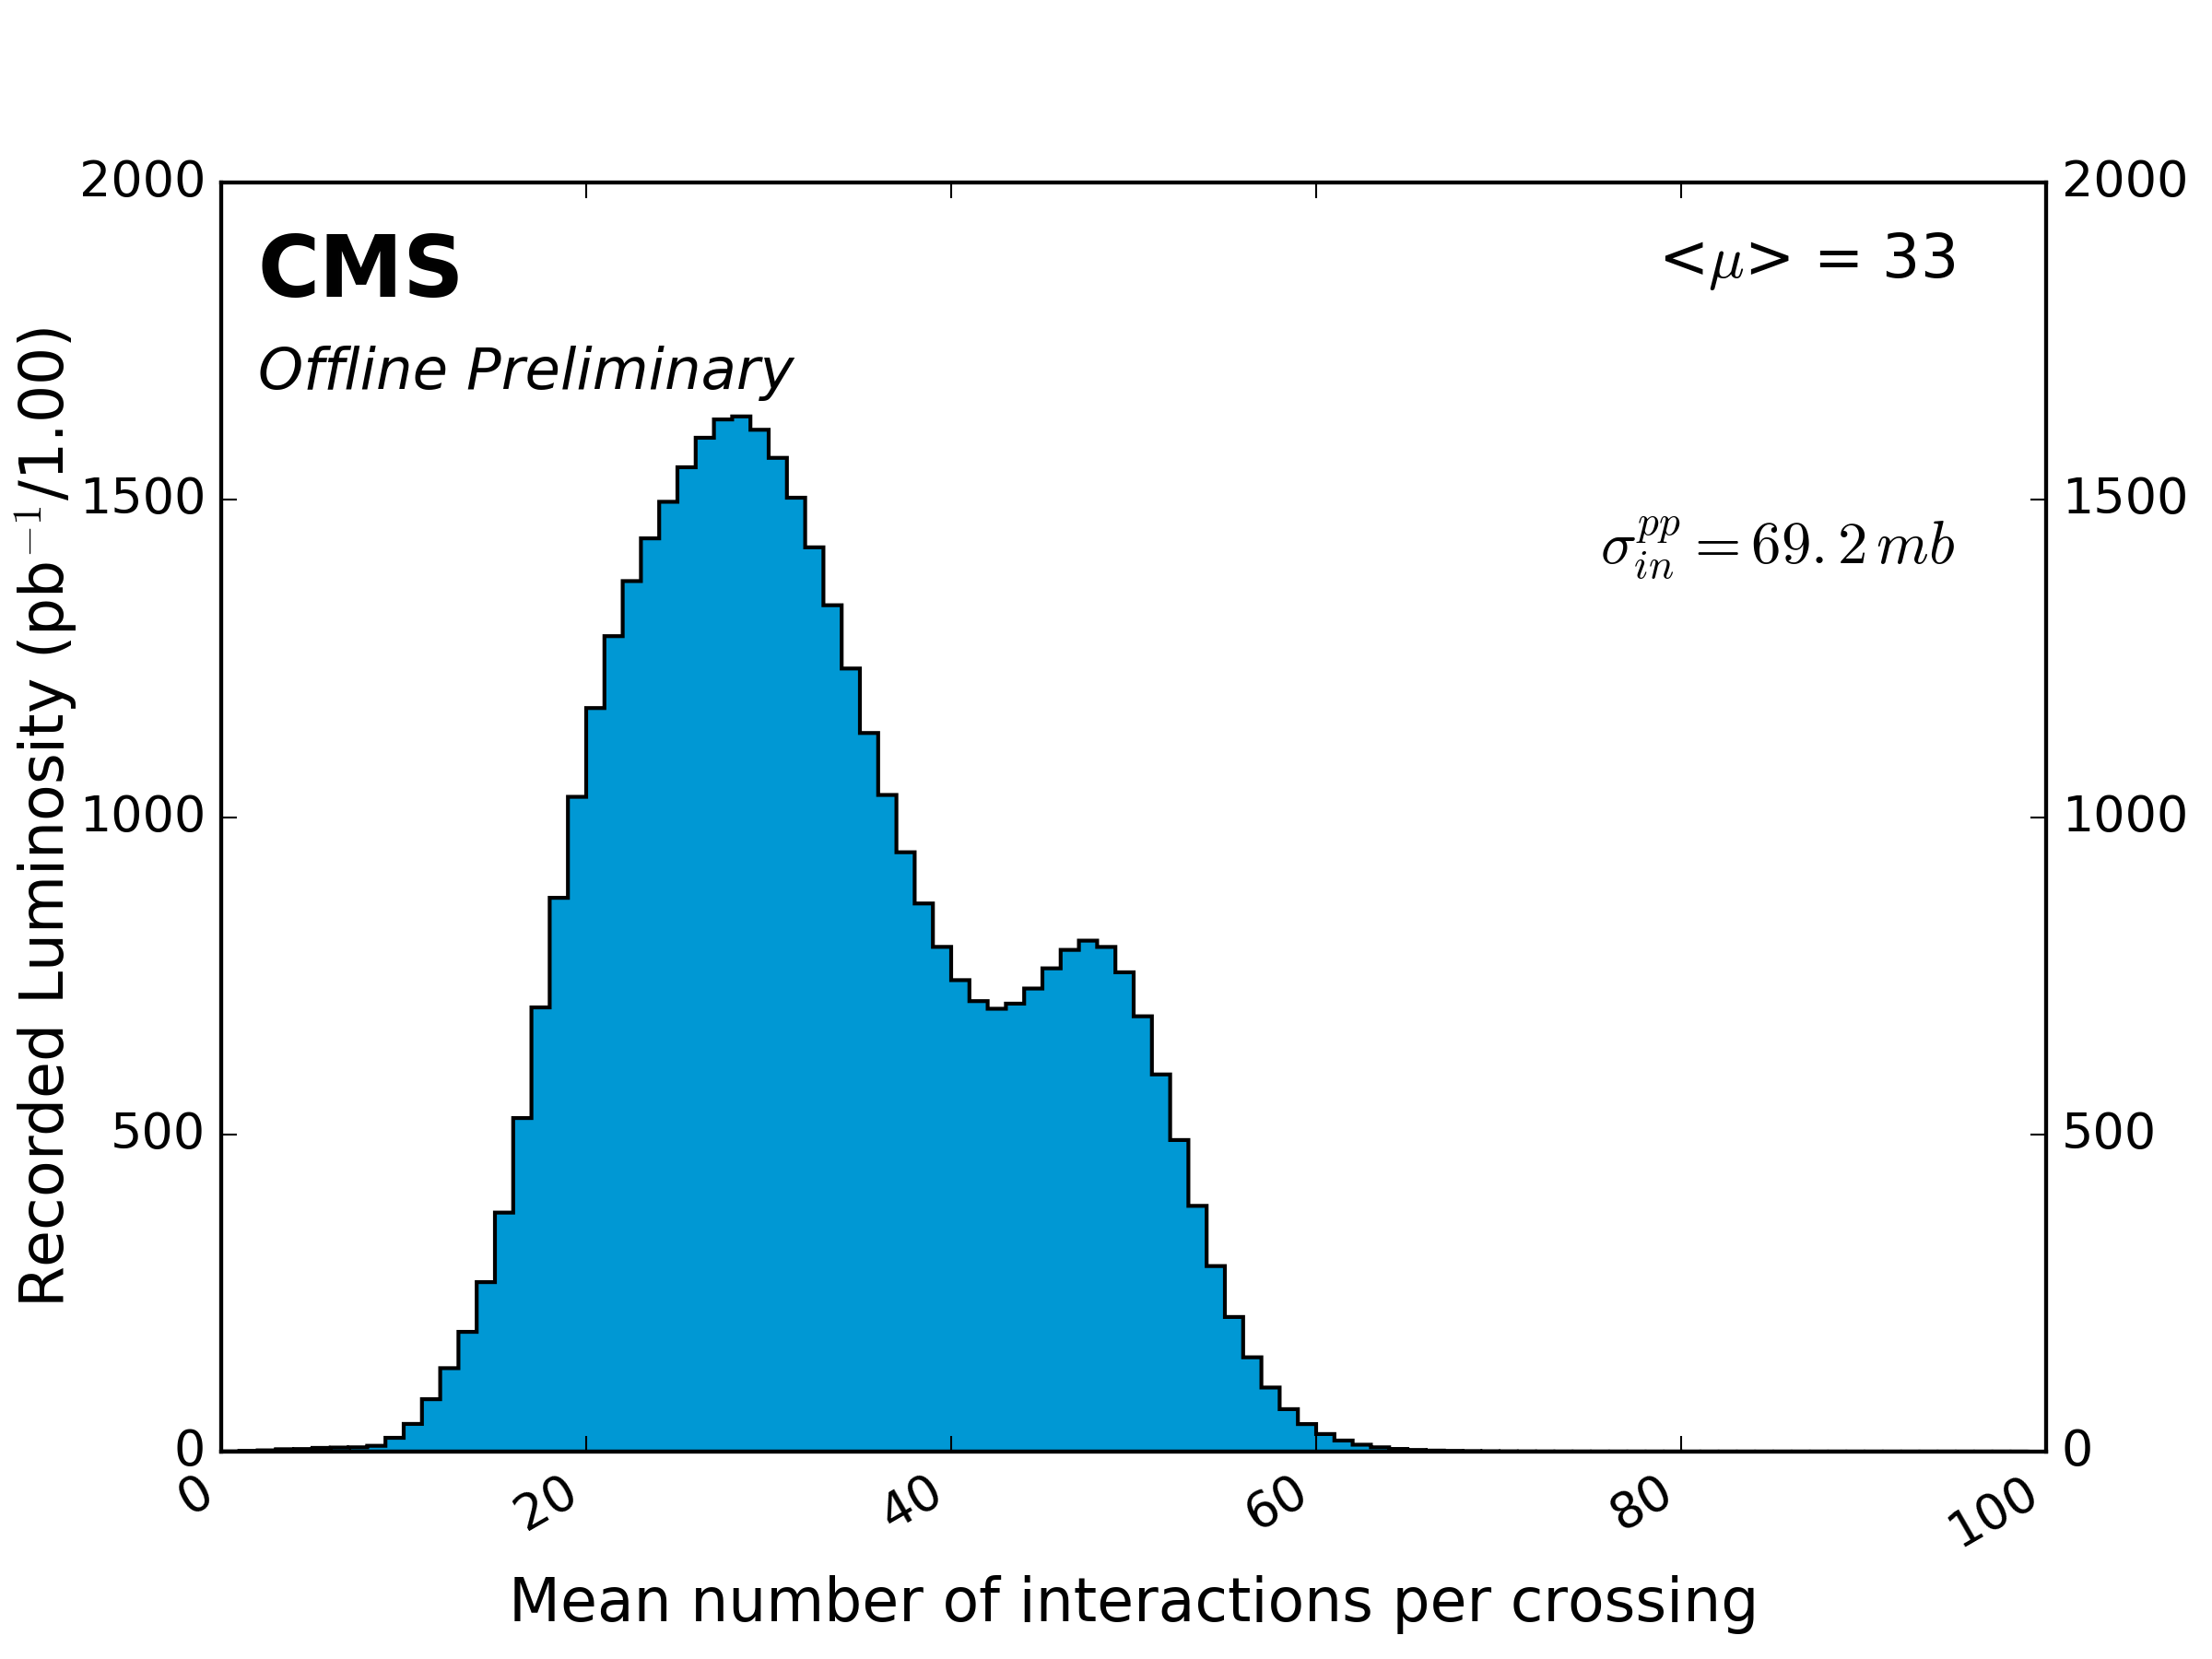
\includegraphics[width=7cm]{thesis_template_cua/Figures/ch5_analysis/pileup_pp_2017_69200_Normtag.png} }}%
    \qquad
    \subfloat[\centering 2018]{{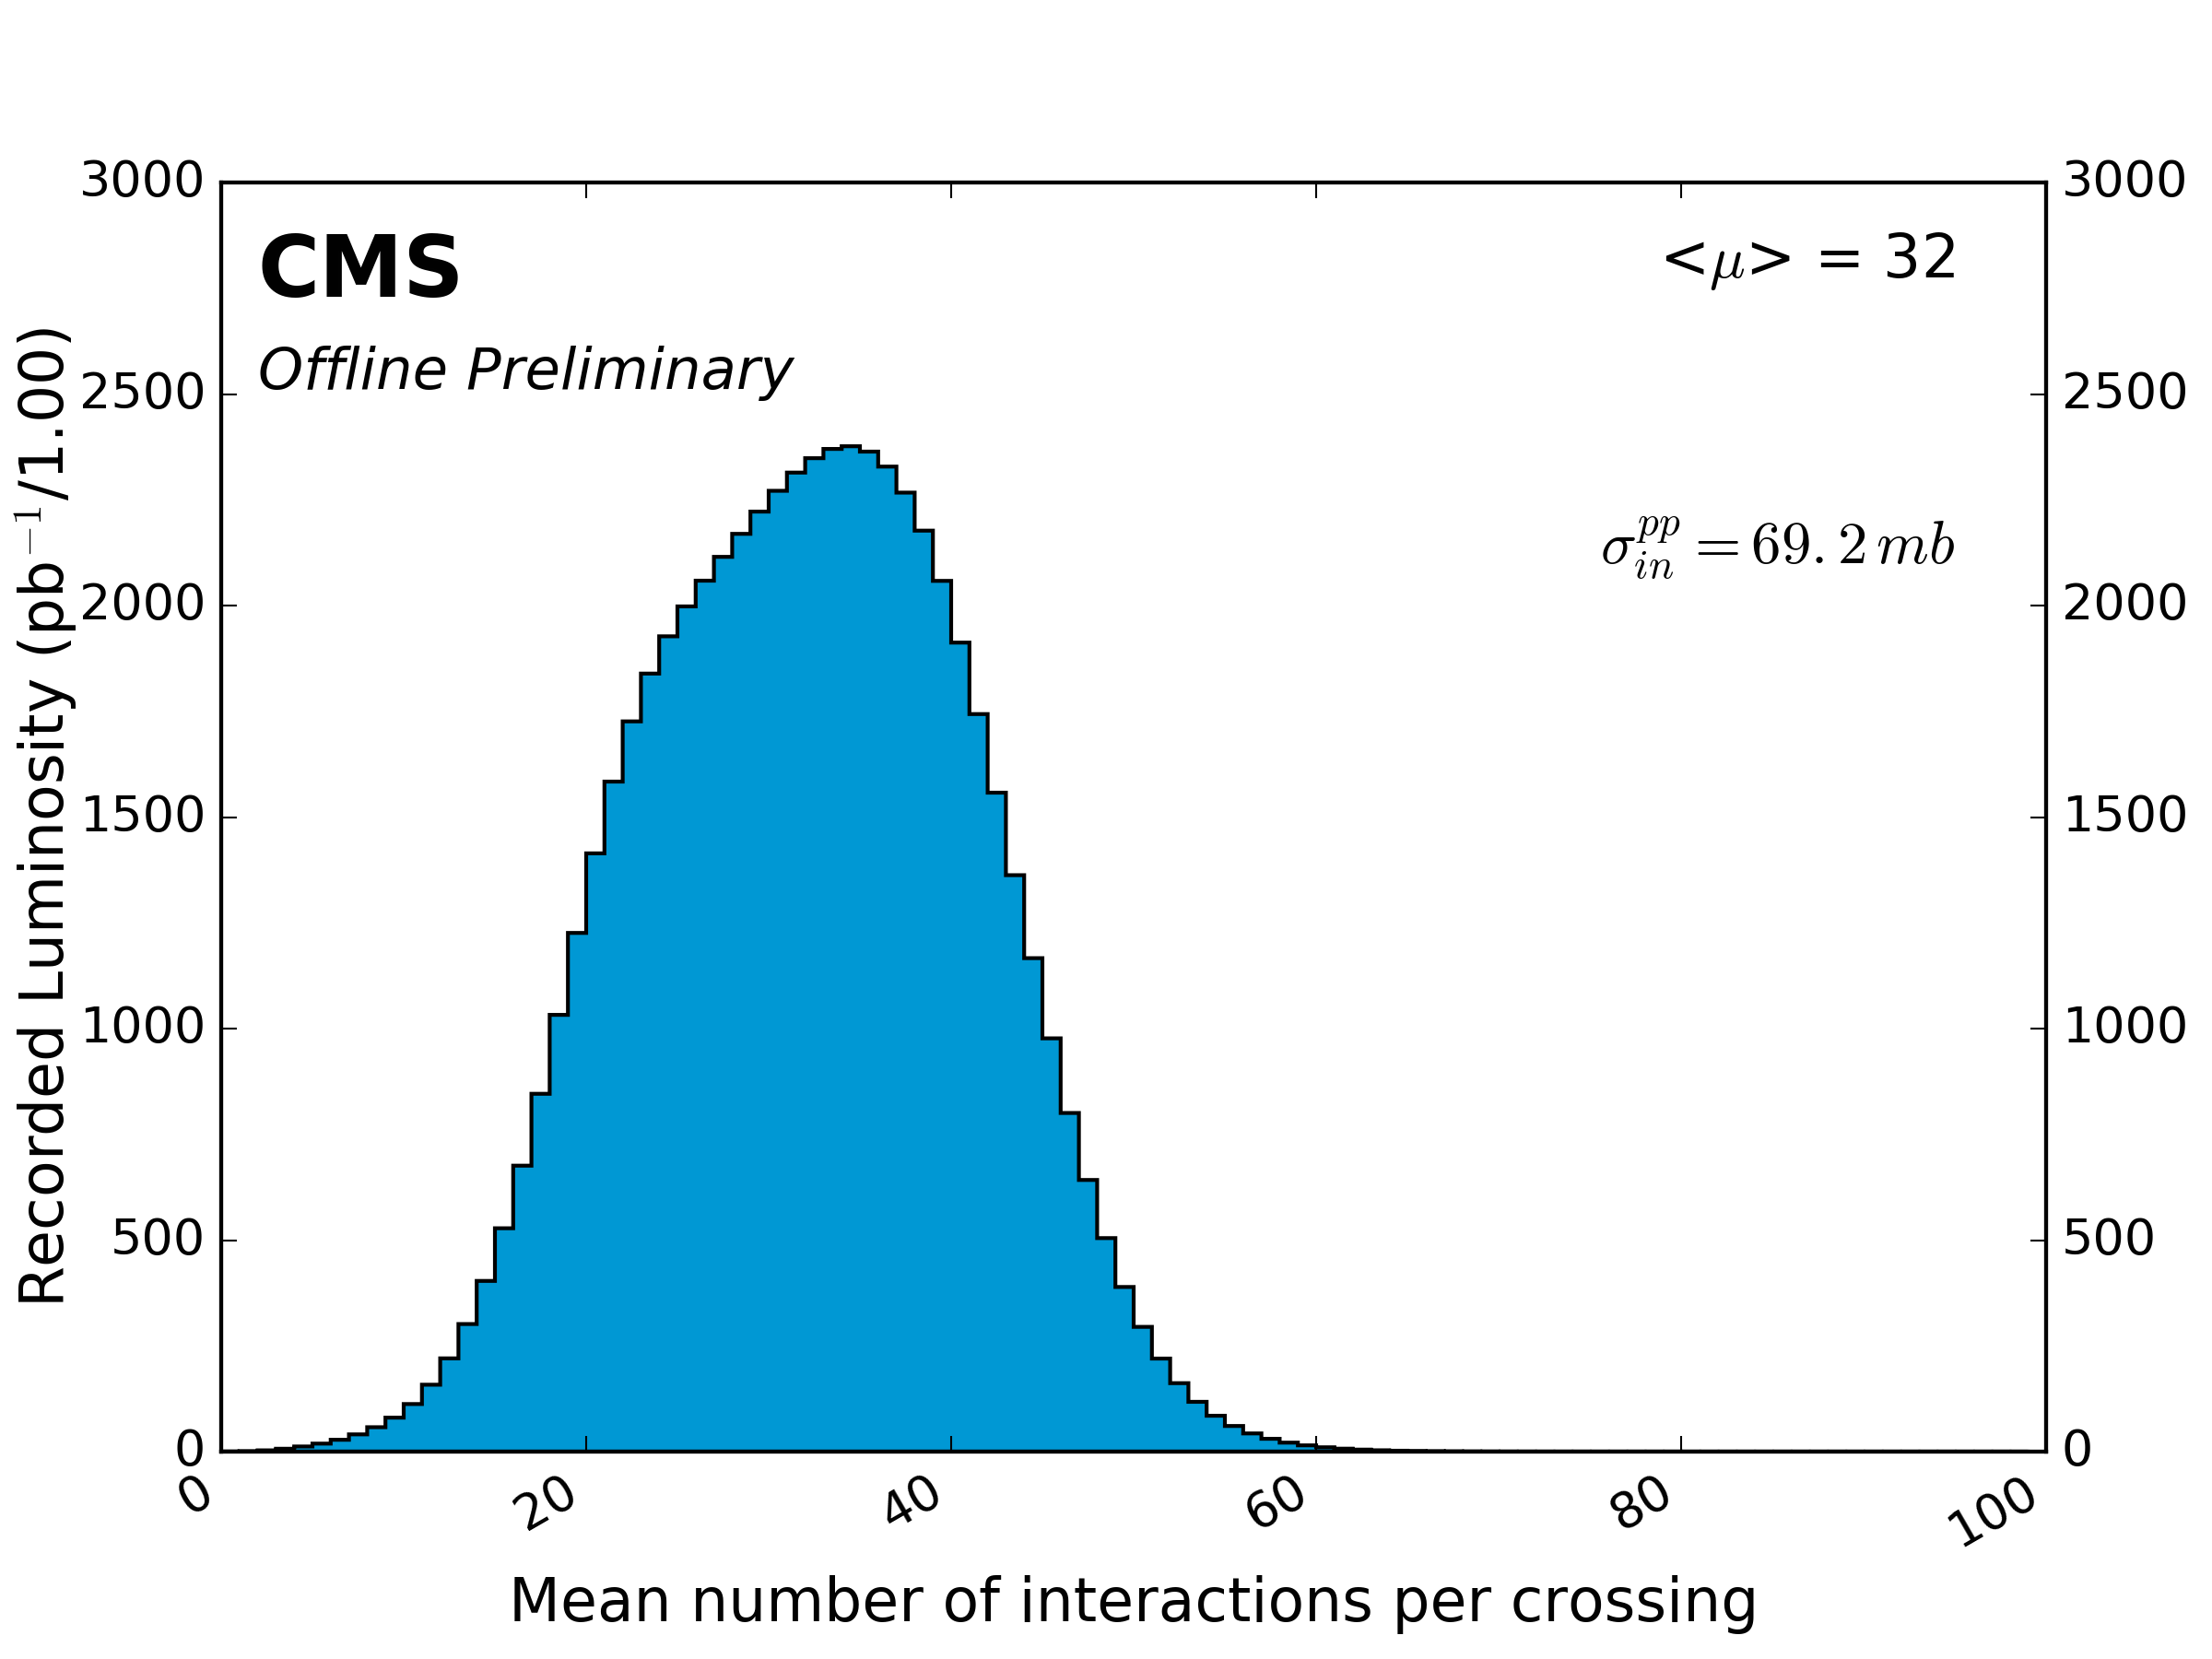
\includegraphics[width=7cm]{thesis_template_cua/Figures/ch5_analysis/pileup_pp_2018_69200_Normtag.png} }}%
    \caption{This figure shows the true pileup distribution of the data observed by the CMS \cite{Chatrchyan:cms_detetectors} for 2016 (a), 2017 (b) and 2018 (c).}%
    \label{analysis:pu_lumipog}%
\end{figure}
The $pileup$ can not be measured directly as it comes from soft $pp$ interaction it is directly correlated to the number of primary vertices ($N_{PV}$). Larger the $N_{PV}$ larger is the pileup. Figure \ref{analysis:pu_lumipog} shows the mean number of interactions per bunch crossing for the year 2016, 2017 and 2018. 

The stream of data recorded by CMS \cite{Chatrchyan:cms_detetectors} is organized into $\bf{Primary \: datasets}$ based on the relevant high level trigger selections as discussed in sections. \ref{l1trigger}, \ref{hlttrigger}. The main ideology behind this organization is to group together events which contain similar physics information. These events are non-exclusive in nature meaning that an event can occur in multiple $primary \;datasets$ based on the HLT selection. In this analysis the datasets relevant to us for single electron final state are EGamma for 2018 and Single Electron $primary \;datasets$ for 2017, 2016 (Pre and Post VFP), and for single muon final state are Single Muon $primary \;datasets$ for 2016 (Pre and Post VFP), 2017 and 2018. Table \ref{tab:data_table} shows the data samples used in for analysis in this thesis.

\begin{table}
\centering
\caption{datasets used in the analysis for all years}
\vspace{3mm}
\scalebox{0.7}{
\begin{tabular}{ll}
%\Xhline{2\arrayrulewidth}
\hline
\hline
Sample&    Cross Section [pb] \\ \hline
\bf{2018} \\ \hline

/EGamma/Run2018A-UL2018\_MiniAODv2\_NanoAODv9-v1/NANOAOD & 1.0 \\
/EGamma/Run2018B-UL2018\_MiniAODv2\_NanoAODv9-v1/NANOAOD & 1.0 \\
/EGamma/Run2018C-UL2018\_MiniAODv2\_NanoAODv9-v1/NANOAOD & 1.0 \\ 
/EGamma/Run2018D-UL2018\_MiniAODv2\_NanoAODv2-v1/NANOAOD & 1.0 \\ 
/SingleMuon/Run2018A-UL2018\_MiniAODv2\_NanoAODv9-v1/NANOAOD  & 1.0\\ 
/SingleMuon/Run2018B-UL2018\_MiniAODv2\_NanoAODv9-v2/NANOAOD & 1.0\\ 
/SingleMuon/Run2018C-UL2018\_MiniAODv2\_NanoAODv9-v2/NANOAOD & 1.0\\ 
/SingleMuon/Run2018D-UL2018\_MiniAODv2\_NanoAODv9-v1/NANOAOD & 1.0\\ \hline

\bf{2017} \\ \hline
/SingleElectron/Run2017B-UL2017\_MiniAODv2\_NanoAODv9-v1/NANOAOD & 1.0\\
/SingleElectron/Run2017C-UL2017\_MiniAODv2\_NanoAODv9-v1/NANOAOD & 1.0\\
/SingleElectron/Run2017D-UL2017\_MiniAODv2\_NanoAODv9-v2/NANOAOD & 1.0\\
/SingleElectron/Run2017E-UL2017\_MiniAODv2\_NanoAODv9-v1/NANOAOD & 1.0\\
/SingleElectron/Run2017F-UL2017\_MiniAODv2\_NanoAODv9-v1/NANOAOD & 1.0\\
/SingleMuon/Run2017B-UL2017\_MiniAODv2\_NanoAODv9-v1/NANOAOD & 1.0\\
/SingleMuon/Run2017C-UL2017\_MiniAODv2\_NanoAODv9-v1/NANOAOD & 1.0\\
/SingleMuon/Run2017D-UL2017\_MiniAODv2\_NanoAODv9-v1/NANOAOD & 1.0\\
/SingleMuon/Run2017E-UL2017\_MiniAODv2\_NanoAODv9-v1/NANOAOD & 1.0\\
/SingleMuon/Run2017F-UL2017\_MiniAODv2\_NanoAODv9-v1/NANOAOD & 1.0\\
/SingleMuon/Run2017G-UL2017\_MiniAODv2\_NanoAODv9-v1/NANOAOD & 1.0\\
/SingleMuon/Run2017H-UL2017\_MiniAODv2\_NanoAODv9-v1/NANOAOD & 1.0\\ \hline

\bf{2016 PreVFP} \\ \hline
/SingleElectron/Run2016B-ver1\_HIPM\_UL2016\_MiniAODv2\_NanoAODv9-v2/NANOAOD & 1.0\\
/SingleElectron/Run2016C-HIPM\_UL2016\_MiniAODv2\_NanoAODv9-v2/NANOAOD & 1.0\\
/SingleElectron/Run2016D-HIPM\_UL2016\_MiniAODv2\_NanoAODv9-v2/NANOAOD & 1.0\\
/SingleElectron/Run2016E-HIPM\_UL2016\_MiniAODv2\_NanoAODv9-v2/NANOAOD & 1.0\\
/SingleElectron/Run2016F-HIPM\_UL2016\_MiniAODv2\_NanoAODv9-v2/NANOAOD & 1.0\\

/SingleMuon/Run2016B-ver1\_HIPM\_UL2016\_MiniAODv2\_NanoAODv9-v2/NANOAOD & 1.0\\
/SingleMuon/Run2016C-HIPM\_UL2016\_MiniAODv2\_NanoAODv9-v2/NANOAOD & 1.0\\
/SingleMuon/Run2016D-HIPM\_UL2016\_MiniAODv2\_NanoAODv9-v2/NANOAOD & 1.0\\
/SingleMuon/Run2016E-HIPM\_UL2016\_MiniAODv2\_NanoAODv9-v2/NANOAOD & 1.0\\
/SingleMuon/Run2016F-HIPM\_UL2016\_MiniAODv2\_NanoAODv9-v2/NANOAOD & 1.0\\ \hline

\bf{2016 PostVFP} \\ \hline
/SingleElectron/Run2016F-UL2016\_MiniAODv2\_NanoAODv9-v1/NANOAOD & 1.0\\
/SingleElectron/Run2016G-UL2016\_MiniAODv2\_NanoAODv9-v1/NANOAOD & 1.0\\
/SingleElectron/Run2016H-UL2016\_MiniAODv2\_NanoAODv9-v1/NANOAOD & 1.0\\

/SingleMuon/Run2016F-UL2016\_MiniAODv2\_NanoAODv9-v1/NANOAOD & 1.0\\
/SingleMuon/Run2016G-UL2016\_MiniAODv2\_NanoAODv9-v1/NANOAOD & 1.0\\
/SingleMuon/Run2016H-UL2016\_MiniAODv2\_NanoAODv9-v1/NANOAOD & 1.0\\ \hline


\hline

%\Xhline{2\arrayrulewidth}
\end{tabular}}
\label{tab:data_table}
\end{table}

The signal and background sample processes were generated using MC simulation. V+Jets background samples were centrally produced at using MADGRAPH5 aMC@NLO \cite{Alwall_2014} generator interfaced  with PYTHIA \cite{Sj_strand_2015} using the CP5  tunes for fragmentation and hadronization. Top samples were produced centrally with  PYTHIA POWHEG using the CP5  tunes for fragmentation and hadronization and Di-Boson (WW, WZ, ZZ) is simulated with PYTHIA8 \cite{Sj_strand_2015}. The last step is passing these events through the CMS detector using Geant4 \cite{Chatrchyan:cms_detetectors} simulation to apply the effects of the detector to the events. Table \ref{tab:bkg_table} shows the list of background samples used in the analysis.

Signal samples were privately produced using MADGRAPH5 aMC@NLO \cite{Alwall_2014} generator interfaced with PYTHIA \cite{Sj_strand_2015} using the CP5  tunes for fragmentation and hadronization. They are generated across a mass grid of the dark matter ($M_{\chi}$) and  mediator mass ($M_{V}$), such that $M_{\chi} < \frac{M_{V}}{2}$. The couplings between the dark matter mediator ($M_{V}$) and quark (q) and dark matter mediation ($M_{V}$) and dark matter particle ($M_{\chi}$) represented by $g_{V,q}$ and $g_{V, \chi}$ are set to 1 and 0.25 respectively, as in the theory paper \cite{Agram_2014}. Each signal sample has around 250k to 300k events and table \ref{tab:signal_table} shows the signal mass grid with their respective cross sections. 
 

\section{Triggers}
\begin{figure} [tpb]
\centering
         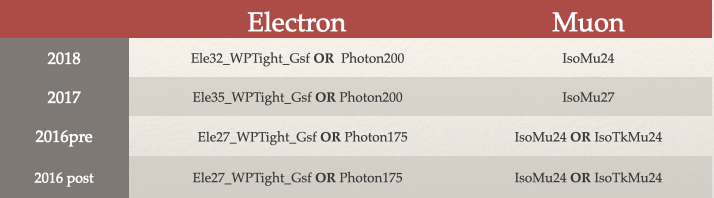
\includegraphics[width=0.8\textwidth,clip=]{thesis_template_cua/Figures/ch5_analysis/triggers.png}
         \vspace*{10mm}
         \caption[Triggers]{This figure show the combination of triggers used in the analysis}
         \label{analysis:triggers}
\end{figure}
This section will present the motivations for selecting a particular HLT path and the specifications of the properties of the selections used in the analysis. The HLT trigger path is a selection mechanism which makes sure that only events which pass the relevant triggers are stored in primary datasets and discarded otherwise. Figure \ref{analysis:triggers} shows the combination of HLTs used in this analysis.

The trigger paths described in Figure \ref{analysis:triggers} are relevant based on the final state signature of the signal sample, which is the presence of an isolated lepton and large missing energy. These paths are dependent on the year in which the data were recorded. Table \ref{tab:trigger table} shows the description of the triggers across different eras. 

In the leptonic analysis, we require the presence of an isolated electron and that is the reason we have used the triggers mentioned in table \ref{tab:trigger table}. In the channel with electron in the final state we require the triggers \verb|HLT_EleYY_WPTight_Gsf_vX| and \\ \verb|HLT_PhotonYY_vX|. The former asks for a trigger level selection of only those events which have an isolated electron in the final state with $p_{T}$ threshold (denoted as \verb|YY|) at 32, 35 and 27 GeV for 2018, 2017 and 2016 (pre \& post VFP) respectively. In latter case, we ask for non-isolated high $p_{T}$ electron with a $p_{T}$ threshold of 200 GeV for 2018 \& 2017 and 175 GeV for 2016 (pre \& post VFP) eras. The reason for choosing the combination of isolated and non-isolated triggers is as follows. Isolation in this context implies the absence of other particles near the electrons, these particles may come from some hadronic activity after collisions. As we move towards selecting high $p_{T}$ electrons the efficiency of the isolated electron trigger drops, this drop is partially accounted by including the non-isolated high $p_{T}$ trigger path. Similarly, we require the presence of an isolated muon in the final state and Table \ref{tab:trigger table} lists the muon channel triggers as well. For collecting such events with final state muons, we require the events to pass \verb|HLT_IsoMuYY_vX| trigger with $p_{T}$ threshold (denoted as YY) of the muon to be 24 GeV for 2016 (pre \& post VFP) \& 2018 and 27 GeV for 2017. We also require the selection of isolated muons with hits in the tracker \verb|HLT_IsoTkMu24_vX| of the CMS detector with a $p_{T}$ threshold of 24 GeV for 2016 (pre \& post VFP) era.

The quantity which allows us to quantify the trigger selections is the efficiency of the HLT path. The efficiency of a trigger path is defined as the ratio of the number of events passing the HLT path and the total number of events that passes the reference trigger selection. The trigger efficiencies are derived for both data sample and the corresponding MC sample for a particular HLT path and since the two efficiencies are different, this effect is propagated to the MC samples through the trigger scale factors. These scale factor is just a ratio of the efficiency of the HLT path in data ($\epsilon_{data}$) with the efficiency of the HLT path in MC ($\epsilon_{MC}$). Figures \ref{analysis:ele_trig} and \ref{analysis:mu_trig} shows the efficiencies for the electron channel HLT paths in table \ref{tab:trigger table} for electrons passing a tight CutBased Id selection and muons respectively.
\begin{table}
\centering
\caption{High Level trigger objects used in the analysis}
\vspace{3mm}
\scalebox{0.9}{
\begin{tabular}{ll}
%\Xhline{2\arrayrulewidth}
\hline
\hline
Signature&    Trigger Name \\ \hline
\bf{Electron Channel}\\

\bf{2018 } \\ \hline
isolated electron & HLT\_Ele32\_WPTight\_Gsf\_vX\\ 
high $p_{T}$ electron & HLT\_Photon200\_vX \\ \hline

\bf{2017} \\ \hline

isolated electron & HLT\_Ele35\_WPTight\_Gsf\_vX\\ 
high $p_{T}$ electron & HLT\_Photon200\_vX \\ \hline

\bf{2016 PreVFP} \\ \hline

isolated electron & HLT\_Ele27\_WPTight\_Gsf\_vX\\ 
high $p_{T}$ electron & HLT\_Photon175\_vX \\ \hline

\bf{2016 PostVFP} \\ \hline

isolated electron & HLT\_Ele27\_WPTight\_Gsf\_vX\\ 
high $p_{T}$ electron & HLT\_Photon175\_vX \\ \hline

\bf{Muon Channel}\\

\bf{2018 } \\ \hline
isolated Muon & HLT\_IsoMu24\_vX\\  \hline

\bf{2017} \\ \hline

isolated Muon & HLT\_IsoMu27\_vX\\  \hline

\bf{2016 PreVFP} \\ \hline

isolated Muon & HLT\_IsoMu24\_vX\\ 
isolated Muon & HLT\_IsoTkMu24\_vX\\\hline

\bf{2016 PostVFP} \\ \hline
isolated Muon & HLT\_IsoMu24\_vX\\ 
isolated Muon & HLT\_IsoTkMu24\_vX\\\hline

\hline

%\Xhline{2\arrayrulewidth}
\end{tabular}}
\label{tab:trigger table}
\end{table}


\begin{figure}%
    \centering

    \subfloat[\centering 2016 Pre VFP]{{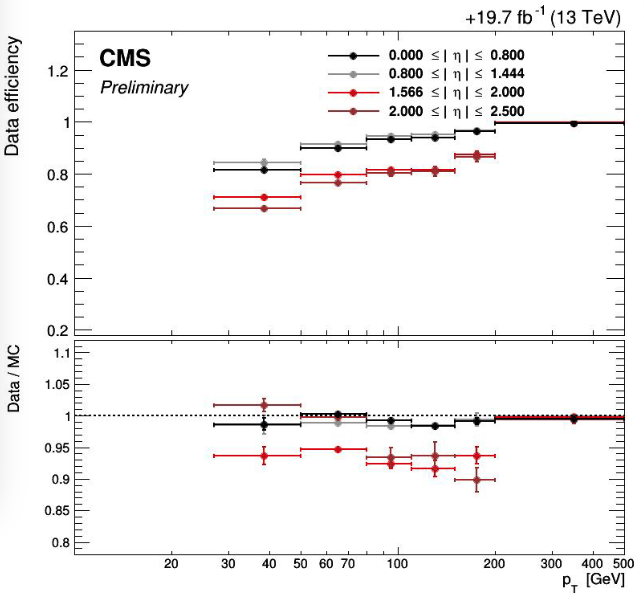
\includegraphics[width=7cm]{thesis_template_cua/Figures/ch5_analysis/ele_2016_pre.png} }}%
    \qquad
    \subfloat[\centering 2016 Post VFP]{{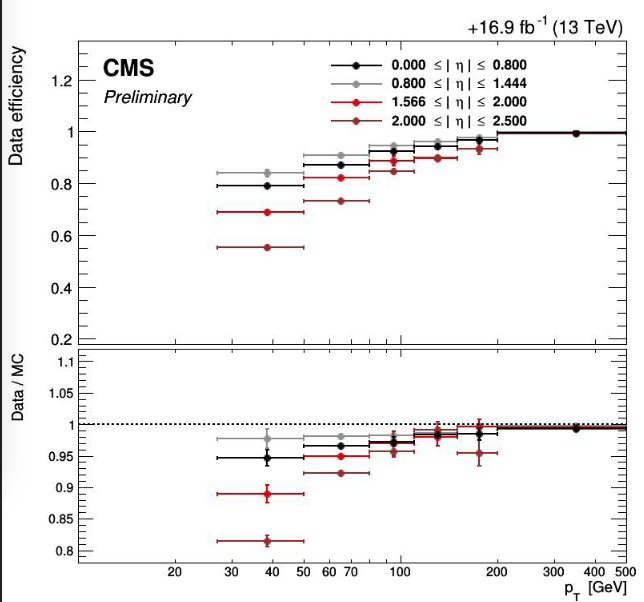
\includegraphics[width=7cm]{thesis_template_cua/Figures/ch5_analysis/ele_2016_post.png} }}%
    \qquad
    \subfloat[\centering 2017]{{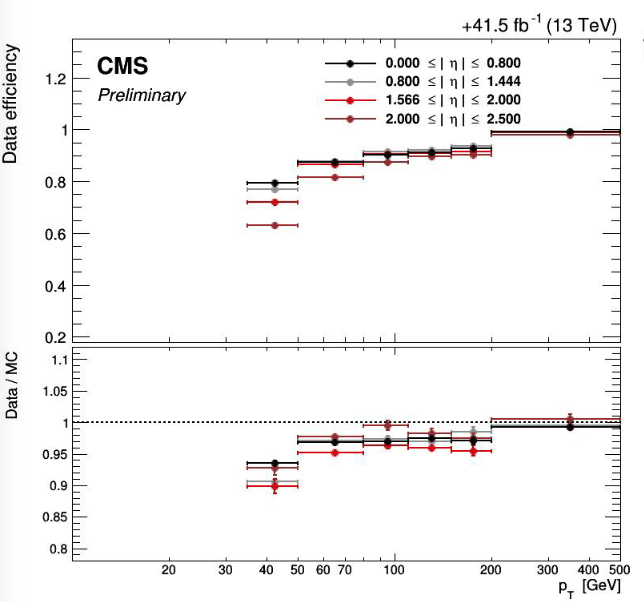
\includegraphics[width=7cm]{thesis_template_cua/Figures/ch5_analysis/ele_2017.png} }}%
    \qquad
    \subfloat[\centering 2018]{{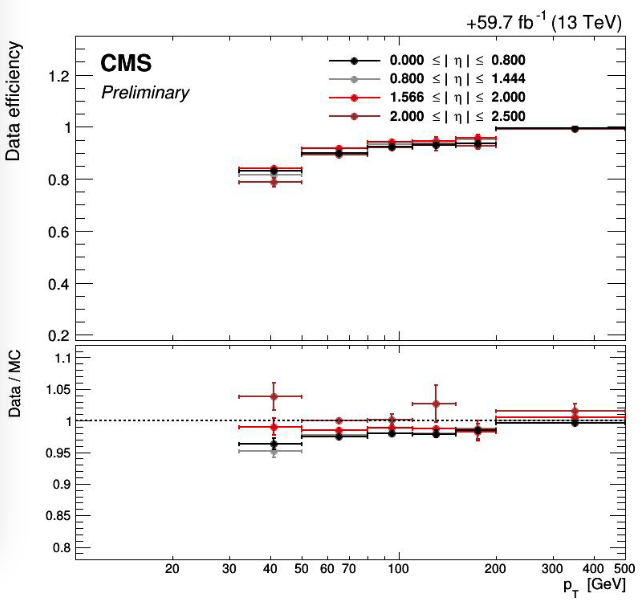
\includegraphics[width=7cm]{thesis_template_cua/Figures/ch5_analysis/ele_2018.png} }}%
    \caption{This figure taken from \cite{eletrigeff} shows the trigger efficiencies as a function of $p_{T}$ for the electron channel HLT paths in Table \ref{tab:trigger table} for electrons passing tightCutbased id for 2016, 2017and 2018 eras.}%
    \label{analysis:ele_trig}%
\end{figure}

\begin{figure}%
    \centering

    \subfloat[\centering 2016 Pre VFP]{{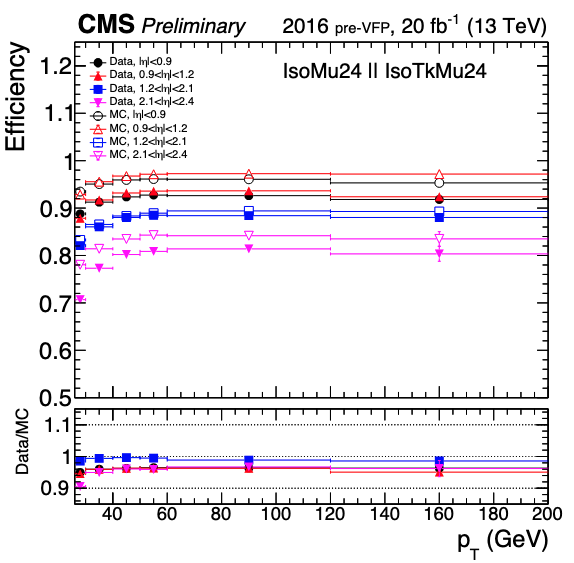
\includegraphics[width=7cm]{thesis_template_cua/Figures/ch5_analysis/mu_2016_pre.png} }}%
    \qquad
    \subfloat[\centering 2016 Post VFP]{{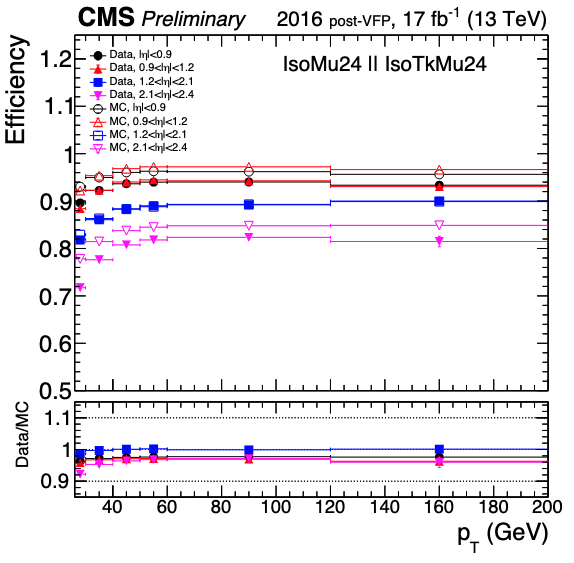
\includegraphics[width=7cm]{thesis_template_cua/Figures/ch5_analysis/mu_2016_post.png} }}%
    \qquad
    \subfloat[\centering 2017]{{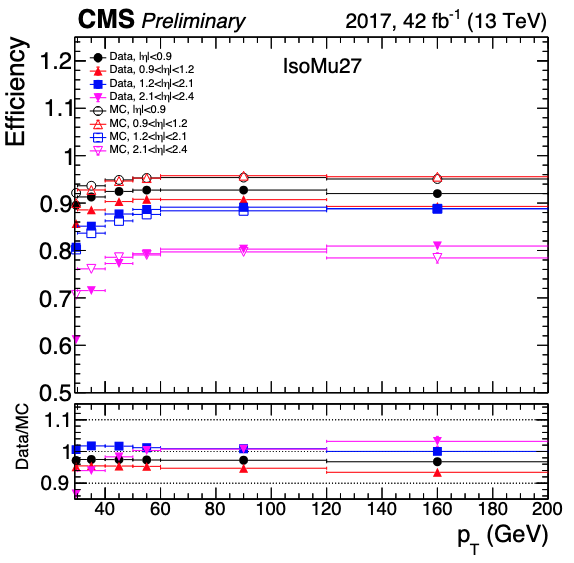
\includegraphics[width=7cm]{thesis_template_cua/Figures/ch5_analysis/mu_2017.png} }}%
    \qquad
    \subfloat[\centering 2018]{{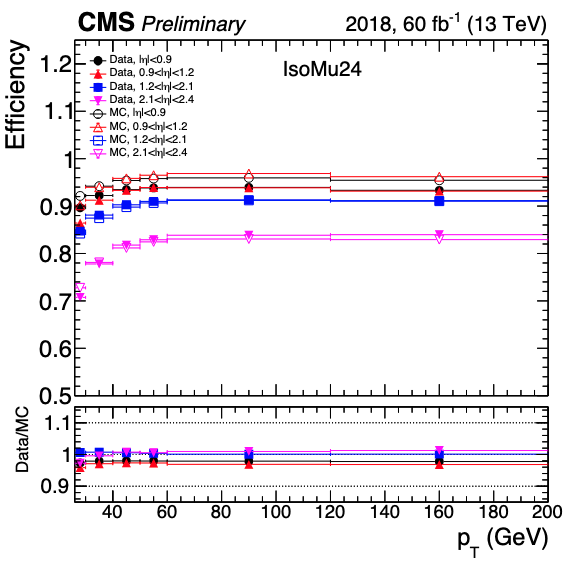
\includegraphics[width=7cm]{thesis_template_cua/Figures/ch5_analysis/mu_2018.png} }}%
    \caption{This figure taken from \cite{muontrigeff} shows the trigger efficiencies as a function of $p_{T}$ for the muon channel HLT paths in Table \ref{tab:trigger table} for 2016, 2017and 2018 eras.}%
    \label{analysis:mu_trig}%
\end{figure}
\section{Object Reconstruction}\label{analysis:objects reconstruction}

\subsection{Electrons}
It is of utmost importance to select electrons which can be reconstructed to gain access to events which provide crucial inference about the interesting physics at the LHC \cite{LHC}. The electrons are charged particles which interact electromagnetically inside the detector, they leave a signature in the form of an energy deposit inside the ECAL, and these energy deposits are matched with the tracks created by hits in silicon tracker to find the kinematical information ($p_{T}, \eta, \phi$) about the electrons \cite{elereco}.

It is important to note that not all electrons produced and detected are of relevance. In order to select relevant electrons we require the electron objects to satisfy certain criteria. So, in this section we will describe the two collections of electrons used in this analysis namely, loose electrons and tight electrons. 

\textbf{Loose Electrons:}

From Table \ref{tab:ele_loose_tight} we can see the selection criteria for selection loose electrons, this criteria basically enhances the efficiency of electron selection (~95\% \cite{cutbasedid}) with a not-so-great identification rate. The $p_{T}$ threshold is set at 15 GeV with a veto \verb|CutBasedID| \cite{cutbasedid}. Alongside these selections, the loose electrons should also satisfy an upper threshold selection of 0.05 in the ECAL barrel (EB) and 0.1 in the ECAL endcap (EC), for the transverse (relative to the primary vertex)  impact parameter $d_{xy}$. A threshold of 0.1 in the ECAL barrel (EB) and 0.2 in the ECAL endcap (EC) on the longitudinal (relative to the primary vertex) impact parameter $d_{z}$ is also required. 

\textbf{Tight Electrons:}

From Table \ref{tab:ele_loose_tight} we can see the selection criteria for selection tight electrons, this criteria basically enhances the selection of electrons with a low mis-identification rate and a rather lower efficiency of electron selection (~70\% \cite{cutbasedid}). The $p_{T}$ threshold is set at 40 GeV with a tight \verb|CutBasedID| \cite{cutbasedid}. Alongside these selections, the tight electrons should also satisfy an upper threshold selection of 0.05 in the ECAL barrel (EB) and 0.1 in the ECAL endcap (EC), for the transverse (relative to the primary vertex)  impact parameter $d_{xy}$. A threshold of 0.1 in the ECAL barrel (EB) and 0.2 in the ECAL endcap (EC) on the longitudinal (relative to the primary vertex) impact parameter $d_{z}$ is also required.

\textbf{ID and Reconstruction Corrections:}

Since in reality the reconstruction and identification of electron objects \cite{elereco} is not perfect inside the CMS detector, corrections for the observed detector effects in recorded data need to be propagated to the MC simulation of the samples. These corrections incorporated through scale factors ($\epsilon_{data} / \epsilon_{MC}$) allow the MC to have similar efficiencies ($\epsilon_{reconstruction}$ \& $\epsilon_{id}$) as the observed data. The scale factors depend on the $p_{T}$ the electron and $\eta$ of the ECAL supercluster and are made available centrally by the respective electron object group for reconstruction and ids for \verb|2018, 2017, 2016 (pre & post VFP))| eras \cite{elerecoid2018}-\cite{elerecoid2016postvfp}. 
\begin{table}
\centering
\caption{Loose and Tight electron selection criteria used}
\vspace{3mm}
\scalebox{0.9}{
\begin{tabular}{llllll}
%\Xhline{2\arrayrulewidth}
\hline
\hline
Type&   $p_{T}$[GeV] &  $|\eta|$ &  Electron ID& $IP_{xy}$ [cm]&$IP_{z}$ [cm]  \\ \hline
\rule{0pt}{4ex}  loose & $>$15 & $<$2.5 & veto ID & 0.05(EB), 0.1(EC) & 0.1(EB), 0.2(EC)\\
\rule{0pt}{4ex} tight & $>$40 & $<$2.5 & tight ID & 0.05(EB), 0.1(EC) & 0.1(EB), 0.2(EC)\\\hline\hline
%\Xhline{2\arrayrulewidth}
\end{tabular}}
\label{tab:ele_loose_tight}
\end{table}




\subsection{Muons}
As discussed before, in the case of a leptonic decay mode of monotop, we require the presence of an electron or a muon in the final state alongside large transverse missing energy. Thus, making muon a critical object for probing the leptonic monotop signature. Analogous to electrons, in this analysis we have used two collections of muons namely, loose muons and tight muons. 
From table \ref{tab:mu_loose_tight}, we see the the $p_{T}$ threshold to be set at 20 GeV for loose muon passing a loose Id and loose isolation selection criteria inside an $|\eta| <$ 2.4 of the CMS detector. Similarly for tight muons, a $p_{T}$ threshold of 40 set for a tight muon passing a tight Id and tight isolation requirement inside an $|\eta| <$ 2.4 of the CMS detector. 

As observed in the efficiencies in the loose and tight ids for electrons, for loose muon Id the selection efficiency is higher than the tight muon Id but the tight muon Id has a lower misidentification rate. From \cite{muidiso}, we see that for loose muon Id the efficiency is less than 99\% with a misidentification rate of less 0.5\%. while for tight muon Id, the efficiency is less than the loose muon Id efficiency at  96\% but a better misidentification rate at 0.3\%.

In order to account for the detector effects in the MC simulation, we need to apply some corrections to the efficiencies of isolation and identification (ID) measurements of the muons in the MC simulation. These corrections are propagated by means of scale factors, they depend on the $\eta$ and $p_{T}$ of the muons. These scale factors are made available centrally through the corresponding muon object group. The id and isolation scale factors are available for \verb|2018, 2017, 2016 (pre & postVFP))| \cite{muidisotwiki}.
\begin{table}
\centering
\caption{Loose and Tight muon selection criteria used}
\vspace{3mm}
\scalebox{0.9}{
\begin{tabular}{llllll}
%\Xhline{2\arrayrulewidth}
\hline
\hline
Type&   $p_{T}$[GeV] &  $|\eta|$ &  muon ID& muon isolation  \\ \hline
\rule{0pt}{4ex}  loose & $>$20 & $<$2.4 & loose ID & loose\\
\rule{0pt}{4ex} tight & $>$40 & $<$2.4 & tight ID & tight\\\hline\hline
%\Xhline{2\arrayrulewidth}
\end{tabular}}
\label{tab:mu_loose_tight}
\end{table}

\subsection{Jets}

\begin{figure} [tpb]
\centering
         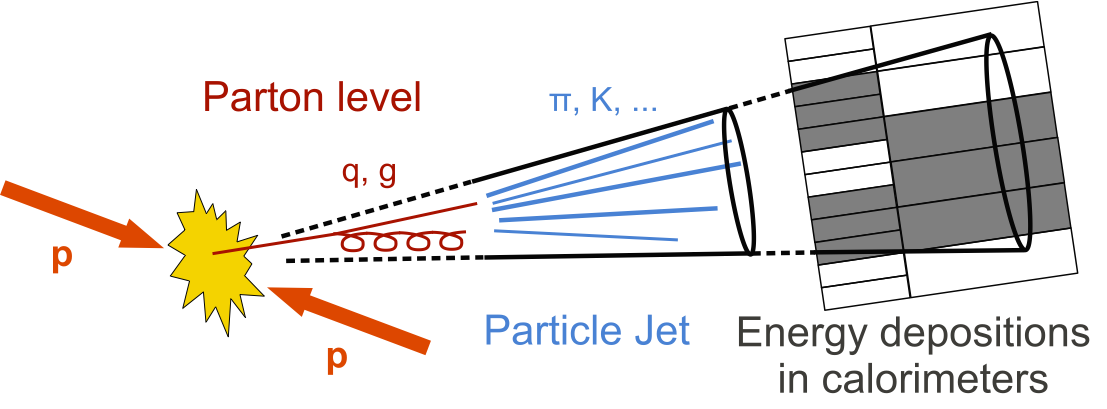
\includegraphics[width=0.8\textwidth,clip=]{thesis_template_cua/Figures/ch5_analysis/jet-hdronization.png}
         \vspace*{10mm}
         \caption[Triggers]{This figure shows the pp collisions resulting in a quark-gluon production which hadronize to produce jets}
         \label{analysis:jets}
\end{figure}
When protons collide at the LHC, quarks and gluons are produced. These particles are color-charged and cannot be isolated due to the color confinement property of strong force. So, the quarks and gluons undergo hadronization and further creating more quark-gluon pair which hadronize futher resulting in a hadronic shower and recorded as a jet signature in the detector. See Figure \ref{analysis:jets}. The collections of jets used in the analysis are the particle-flow charged hadron subtraction jets (AK4 PF Jets) with a cone radius of 0.4 cm in the $\eta$-$\phi$ plane of the CMS detector. We will also look at the AK4 Jets tagged as coming from the hadronization of a b-quark. 


\subsubsection{AK4 PF CHS Jets}
First, to understand the naming of these jets as \verb|AK4 PF CHS| Jets. Jets are reconstructed by clustering the energy deposits in the ECAL with the tracks in the silicon tracker (also know as PF candidates as they are constructed by the Particle Flow algorithm \cite{pfalgo}), CMS uses the algorithm named anti-$k_{T}$ (AK) algorithm \cite{antikt_algo} to cluster jets with a jet radius of 0.4 cm. The effects of pileup are handled by the Charged Hadronic Subtraction (CHS) algorithm \cite{chsalgo}.

In the anti-$k_{T}$ clustering algorithm the distance between object is measured by the equation \ref{eqn:eqlabel}. Where $\Delta_{ij}^{2p}$ = $\left(y_{i} - y_{j}\right)^{2p}$ + $\left(\phi_{i} - \phi_{j}\right)^{2p}$, $k_{ti}$, $y_{i}$, and $\phi_{i}$ are respectively the transverse momentum,
rapidity and azimuth of particle $i$. $d_{ij}$ refers to the distance between the objects $i$ and $j$ which $d_{iB}$ refers to the distance between the object $i$ and the Beam. The reason behind the naming of the algorithm anti-$k_{T}$ (p$<$0) is to differentiate from the already existing $k_{T}$ algorithm (p$>$0).
\begin{equation}
\label{eqn:eqlabel}
d_{ij} = min\left(\frac{1}{d_{ti}^{2p}}, \frac{1}{d_{tj}^{2p}}\right) \frac{\Delta_{ij}^{2p}}{R^{2}}, \:\: d_{iB} = \frac{1}{k_{ti}^{2}}
\end{equation}

The performance of reconstructed jets is different in data and in simulated samples. Because of the presence of detector effects the reconstruction of true physical jets is inaccurate in both data and simulated samples. To account for these effects a correction is derived using a multijet event sample \cite{jecjer}. There are two type of jet corrections that are applied (as a function of jet $\eta$ and $p_{T}$) in this analysis, the jet energy scale (JES) and the jet energy resolutions (JER). The JES correct the $p_{T}$ of the jets, while the JERs correct the resolution of the simulated samples to match with data \cite{jecjer}, the JER and JES are combinedly called as jet energy corrections or JEC for short. More details in section \ref{jer} and \ref{jes}

Prior to applying the JEC (JER/JES), the jets have to pass a selection criteria in order to ensure that the reconstructed jets correspond to the real physics jets \cite{good-jets}. The identification criteria is shown in figure \ref{analysis:jet-id} for 2016, 2017 \& 2018 eras:

\begin{figure}%
    \centering

    \subfloat[\centering 2016]{{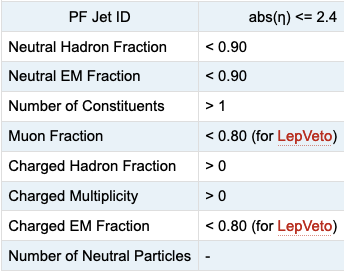
\includegraphics[width=7cm]{thesis_template_cua/Figures/ch5_analysis/2016-jetid.png} }}%
    \qquad
    \subfloat[\centering 2017/2018]{{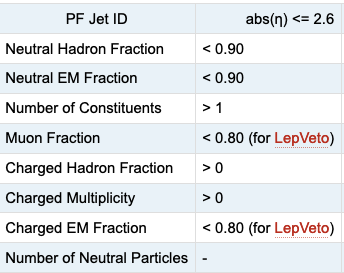
\includegraphics[width=7cm]{thesis_template_cua/Figures/ch5_analysis/2017-18-jetid.png} }}%
    \qquad
    \caption{This figure taken from \cite{jetidentification} shows the identification criteria for jet selection}%
    \label{analysis:jet-id}%
\end{figure}

After this selection criteria the analysis also employs a $p_{T}>$ 30 GeV selection on the jets. In order to account to effect of particles inside the jet due to pileup, a pile tight JetId is used as discriminator on jets with $p_{T}< 50$ GeV. It is BDT discriminator which is used to distinguish the prompt jets from the pileup jets \cite{puid}.
\subsubsection{JER}\label{jer}
The JER corrections help in adjusting the resolution in simulated samples to match with the resolution data. There can be two scenarios for updating the resolution (4 momentum) of the jet, one where a particle level jet is found around the reconstructed jet such that the distance between the two jets $\Delta R < R/2$, and the other, where the particle-level jet can not be found within $\Delta R < R/2$. The correction formulae are shown in eq \ref{eqn:jer1} and \ref{eqn:jer2} respectively for the two cases. where $s_{JER}$ is the resolution scale factor, $p_{T}$ is the transverse momenta of the reconstructed jet and $p_{T}^{particle}$ is the the transverse momenta of the particle-level jet, $\mathcal{N}\left(0, \sigma_{JER}\right)$ is Gaussian normal distribution with mean 0 and standard deviation $\sigma_{JER}$. 

These correction factors are applied as a function of the $\eta$ and $p_{T}$ of the reconstructed jet and are provided centrally by the CMS collaboration \cite{jersf}

\begin{equation}
\label{eqn:jer1}
c_{JER} = 1 + \left(s_{JER} - 1\right)\frac{p_{T}-p_{T}^{particle}}{p_{T}}
\end{equation}

\begin{equation}
\label{eqn:jer2}
c_{JER} = 1 + \mathcal{N}\left(0, \sigma_{JER}\right)\sqrt{max\left(s_{JER}^{2} - 1, 0\right)}
\end{equation}
\subsubsection{JES}\label{jes}
The jet energy scale corrections are applied via a factorized method meaning that it is a step by step process to counter different effects. At each factorized step a correction factor is applied to the jets as a function of $\eta$ \& $p_{T}$. The first step involves accounting for the contribution from soft collisions to the jets, also known as pileup. Following which the detector effects are taken into consideration, the differences are approximated as a function of $\eta$ \& $p_{T}$. These correction are provided centrally by the CMS collaboration \cite{jersf}.
\subsubsection{AK4 Heavy flavor tagged PF CHS Jets}
As discussed in section \ref{analysis-strategy}, that the final state signature in mono-top requires the presence of a lepton, a b-tagged jet and large missing energy. A b-tagged jet is jet coming from hadronization of b-quark, CMS uses the DeepJet algorithm \cite{Bols_2020} which a neural network based model for classification of the jet based on the working points in table \ref{tab:btagwp}. In this analysis we have used the medium working point and the corresponding corrections are applied and uncertainties propagated.

As we have understood from previous sections that in order for the simulated samples to behave similar to data we need to update the efficiencies of the simulated samples to match with data. a scale factor is derived as the ratio of efficiency of data with the MC sample. These scale factors depend on jet $p_{T}$, $\eta$ and hadron flavor of the jet at generator level.

As you will see in section \ref{event-selection} we have 
\begin{table}
\centering
\caption{b-tag working points used in the analysis}
\vspace{3mm}
\scalebox{1}{
\begin{tabular}{lllll}
%\Xhline{2\arrayrulewidth}
\hline
\hline
Working Point&   discriminant value $\geq$&  Mistag Probability \\ 
&2016\,  \,2017\,   \,2018\,&\\\hline
\rule{0pt}{4ex}  loose & 0.0614 0.0521 0.0494 & 10\% \\\hline
\rule{0pt}{4ex}  medium & 0.3093 0.3033 0.2770 & 1\% \\\hline 
\rule{0pt}{4ex}  tight & 0.7221 0.7489 0.7264 &0.1\% \\\hline

%\Xhline{2\arrayrulewidth}
\end{tabular}}
\label{tab:btagwp}
\end{table}

\subsection{Missing Transverse Energy}
The CMS detector has many cylindrical layers which provides a hermetic coverage to technically detect all the particles produced during p-p collisions. It is because of this property of the CMS detector which makes it possible to measure the kinematic properties of all the particles produced. Since the collisions take place in the rest frame of the beam, the net transverse momenta of the beam is zero i.e. the total transverse momenta vector $\bf{p_{T}^{miss}}$ of the outgoing particles should be zero by the law of conservation of momentum. However, some particles like the neutrinos or the hypothesized dark matter particles are not detected by the CMS detector which results in a non-zero net transverse momenta $\bf{p_{T}^{miss}}$. So, $\bf{p_{T}^{miss}}$ is used as a probe for such weak-interacting particles.

The reconstruction of the missing energy $\bf{p_{T}^{miss}}$ is done using the PF candidates analogous to the the jet reconstruction. As is known that the reconstruction efficiency is affected by the detector and the mis-reconstruction effects, a correction factor is introduced which propagates the corrections applied to jets (ref \ref{jer} and \ref{jes}) to the missing energy as in eq \ref{eqn:metcorr}, these corrections are also know as Type I corrections.



\begin{equation}
\label{eqn:metcorr}
p_{T}^{miss, corr} = p_{T}^{miss} - \sum_{jets}\left(p_{T, jet}^{corr}-p_{T, jet}\right)
\end{equation}

On top of the Type I corrections, met x-y shift corrections \cite{metxy} are applied to the missing energy. These corrections help in correcting the azimuthal ($\phi$) angle dependence on the reconstructed met to combat the effects of an-isotropic detector response, detector mis-alignment and displacement of the beam spot. 

Large missing energy may not always point to interesting physics phenomena but may also act as a proxy for uninteresting effects such as detector noise, cosmic rays and beam-halo particles. Such met is called \verb|fake met , false met or anamolous met|. So, we have used some algorithms which use timing, pulse-shape and signal topology to identify and remove false met. The filters \cite{metfilters} in tab \ref{tab:metfilter} have been recommended to remove fake met and are applied to both data and MC.

\begin{table}
\centering
\caption{Met Filters used in the analysis}
\vspace{3mm}
\scalebox{0.8}{
\begin{tabular}{lllll}
%\Xhline{2\arrayrulewidth}
\hline
\hline
Filter name&   2016 (pre \& postVFP) &  2017 &  2018 \\ \hline
%\rule{0pt}{4ex}  loose & $>$20 & $<$2.4 \\
\rule{0pt}{4ex} \bf{primary vertex filter:}
& \checkmark & \checkmark  & \checkmark \\
removes events without reconstructed primary vertices\\ \hline
\rule{0pt}{4ex} \bf{beam halo filter:}\\  
removes beam halo backgrounds& \checkmark & \checkmark  & \checkmark \\\hline

\rule{0pt}{4ex} \bf{HBHE noise filter:} & \checkmark & \checkmark  & \checkmark \\
removes events with poor HCAL performance in general\\\hline

\rule{0pt}{4ex} \bf{HBHEiso noise filter:} \\
removes events with poor isolated HCAL channels& \checkmark & \checkmark  & \checkmark \\\hline
\rule{0pt}{4ex} \bf{EcalDeadCellTriggerPrimitiveFilter:}\\
removes events with dead ECAL channels that fired HLT triggers& \checkmark & \checkmark  & \checkmark \\\hline
\rule{0pt}{4ex} \bf{Bad PF Muon Filter}  \\
removes events with poor PF muon reconstruction& \checkmark & \checkmark  & \checkmark \\\hline
\rule{0pt}{4ex} \bf{Bad PF Muon Dz Filter:}\\
& \checkmark & \checkmark  & \checkmark \\\hline
\rule{0pt}{4ex} \bf{ee badSC noise filter}  & \checkmark & \checkmark  & \checkmark \\\hline
\rule{0pt}{4ex} \bf{ECAL bad calibration filter update}  & \checkmark & \xmark  & \xmark\\\hline


%\Xhline{2\arrayrulewidth}
\end{tabular}}
\label{tab:metfilter}
\end{table}


\section{Efficiency Studies}
\subsection{Lepton Identification}
jijiji
\section{Event Selection}\label{event-selection}
In this section, we will describe in detail the selection criteria on the events which maximize the contribution of signal like events in the signal region and quantify major backgrounds (as discussed in section \ref{analysis-strategy} in the control region regions dominated by W+Jets and $t\Bar{t}$ backgrounds, respectively.

The distinguishing variable used between signal and background like events is the transverse mass of W boson 
\ref{mtw}. This variable allows for compare events dominated by signal-like events and identify the signal like signature in the signal region with a characteristic shape different from the background like events. As we require the presence of a single b-tagged jet, a lepton and large met in the signal region, on top of the basic event selection (pre-selection) we use the number of b-tagged jets selection criteria to differentiate between the signal and background control regions.

This section will first describe the basic selection criteria for event selection, followed by the background control region and signal region definitions.

\begin{equation}\label{mtw}
m_{T}^{W} = \sqrt{2 p_{T}^{l} \cancel{\it{E}}_{T}(1 - cos(\Delta\phi(l - \cancel{\it{E}}_{T})))}
\end{equation}
\subsection{Pre-Selection}
As discussed in the section \ref{analysis-strategy}, the signal region is dominated by the presence of large missing energy from the DM candidate decay an isolated lepton and a b-tagged jet which come from the decay of the single top quark. The top quark recoils against the DM candidate before decaying into a b-tagged jet and a W boson. The W boson further decays into a lepton and its corresponding anti-neutrino. The mono-top signal signature of consist of a single high $p_{T}$ jet which is tagged as a originating from the hadronization of a B hadron. See sec \ref{ch4:btagging} on how to classify a jet as a b-jet.

\begin{enumerate}
  \item The magnitude of missing transverse momentum of the W boson $m_{T}^{W}>$150 GeV. As the phase space for $<150$ GeV would be covered by the hadronic monotop channel \cite{hadronicpaper}. In addition, we also require the presence of isolated leptons which pass the tight identification criteria as defined in section \ref{analysis:objects reconstruction} and an isolated $high-p_{T}$ jets ($p_{T}>70$ GeV) with radius of 0.4 cm recoiling against the DM candidates. These AK4 jets would later be tagged as b-jets and used as a discriminant between the signal and background control regions.
  
  \item The angle between missing energy and leading AK4 Jet in transverse plane of the detector i.e. $\Delta\phi(\cancel{\it{E}}_{T}, Jet)>$ 1.5. This selection removes the mis-modelled signal region in the detector. The mis-modelling is the result of QCD events for which the momenta measurements are incorrectly measured.
  
  \item The missing transverse momentum $\cancel{\it{E}}_{T}>$ 100 GeV to only consider region of the phase space which are well modelled in the simulation.

  \item In the 2018 data taking period, due to power failure of a 40$^{\circ}$  section of one end of the Hadronic Calorimeter (HEM) so the events in data collected from this particular region of the detector have to be removed. The events with missing energy ($\cancel{\it{E}}_{T}>$ 470 GeV) pointing to the region -0.62 $<\phi(\cancel{\it{E}}_{T})<-1.62$ are veto'd. Also, jets with $p_{T}>30$ in the previously mention HEM region and -3 $<\eta<$-1.3 are also not considered in the analysis.
\end{enumerate}

\subsection{Background Control Regions}
As mentioned in sec \ref{analysis-strategy}, W+jets and $t\Bar{t}$ are the major backgrounds which could possibly mimic the monotop signature. It is very essential to quantify the estimation of these backgrounds to get a precise estimate of them in the signal region. The number of b-tagged jets is used a differentiating object between the signal and background control region. In the signal region we require the presence of exactly one b-tagged jet which for W+jets and $t\Bar{t}$ we require zero and at least two b-jets, respectively.
\subsubsection{W Control Region}
\subsubsection{Top Control Region}
\subsection{Signal Region}
\subsection{Event Yields}

\section{Systematic Uncertainties}
this is very important

\section{Statistical Analysis}

\section{Results}
\chapter{Conclusion}
\label{chapter:conclusion}


\section{An Interesting Section}

Great thoughts that further your argument. This includes lots of strong evidence presented throughout several paragraphs, each accompanied by necessary citations.
\begin{quotation}
    \noindent Here is a block quotation---a passage from a text you found insightful and wanted to share with others. Maybe it is from a journal article, website, or book. Irrespective, it should support the argument being made.\footnote{A citation for the quoted material.}
\end{quotation}
Maybe a sentence or two that bring the argument and evidence together.\citep{dos_santos_2020}



\section{Another Insightful Section}

More ideas that really make this a great paper. Maybe a footnote or two.\footnote{Some peripheral thoughts that belong in a note.}



\backmatter

\bibliographystyle{unsrt}
\bibliography{backmatter/refferences}

    \begin{appendixes}
    \chapter{Chapter 1}\label{appendix: chapter1}

\begin{figure}
\centering
         
\includegraphics[width=0.5\textwidth,clip=]{Figures/Introduction/CUA_logo_2.png}
         \caption{CUA Logo 2}
         \label{CUA-logo-2}
\end{figure}
    \end{appendixes}

    \begin{appendixes}
    \chapter{Chapter 2}\label{appendix: chapter2}

\lipsum[4-5]
    \end{appendixes}
    
    \begin{appendixes}
    \chapter{Chapter 3}\label{appendix: chapter3}

\lipsum[4-5]
    \end{appendixes}
    

\end{document}
